% Sample LaTeX file for creating a paper in the Morgan Kaufmannn two
% column, 8 1/2 by 11 inch proceedings format.
\documentclass{article} % For LaTeX2e
\usepackage{nips14submit_e,times}
\usepackage{hyperref}
\usepackage{url}
\usepackage{amsmath,amsthm}
\usepackage{graphicx}
\usepackage{bm}
\usepackage{hyperref}
\usepackage{natbib}
\usepackage{fancyhdr}
\usepackage{latexsym,amsbsy,amssymb,color,xspace,booktabs}

% genereal purpose macros here
\newcommand{\marg}{\marginpar}
\newcommand{\todo}[1]{{\color{red}{TODO: #1}}}
\newcommand{\commentOut}[1]{} 
\newcommand{\add}[1]{\textcolor{red}{#1}} % To highligh modified text

% abbreviations
\newcommand{\etal}{et al.\xspace}
\newcommand{\ie}{i.e.\xspace}
\newcommand{\eg}{e.g.\xspace}
\newcommand{\Ie}{I.e.\xspace}



% Matrices and vectors 
\newcommand{\mat}[1]{\mathbf{#1}}
\renewcommand{\vec}[1]{ \mathbf{#1} } % math bold
\newcommand{\vecS}[1]{\boldsymbol{ #1 }  } % this for boldsymbols
\newcommand{\vecentry}[2]{{\mathrm #1_{#2}}}
\newcommand{\matentry}[3]{{\mathrm #1_{#2,#3}}}
\newcommand{\matcol}[2]{\mat{#1}_{\cdot #2}}
\newcommand{\matrow}[2]{\mat{#1}_{#2 \cdot}}

 % Matrices here
 \newcommand{\A}{\mat{A}}
\newcommand{\B}{\mat{B}}
\newcommand{\C}{\mat{C}}
\newcommand{\D}{\mat{D}}
\newcommand{\F}{\mat{F}}
\newcommand{\G}{\mat{G}}
\newcommand{\I}{\mat{I}}
\renewcommand{\L}{\mat{L}}
\newcommand{\X}{\mat{X}}
\newcommand{\W}{\mat{W}}
\newcommand{\Y}{\mat{Y}}
\newcommand{\Z}{\mat{Z}}
\renewcommand{\S}{\mat{S}}
\newcommand{\K}{\mat{K}}
\newcommand{\U}{\mat{U}}

% Vectors here
\newcommand{\f}{\vec{f}}
\newcommand{\g}{\vec{g}}
\newcommand{\h}{\vec{h}}
\newcommand{\m}{\vec{m}}
\renewcommand{\t}{\vec{t}}
\renewcommand{\u}{\vec{u}}
\renewcommand{\v}{\vec{v}}
\newcommand{\w}{\vec{w}}
\newcommand{\x}{\vec{x}}
\newcommand{\y}{\vec{y}}
\newcommand{\z}{\vec{z}}
\newcommand{\s}{\vec{s}}

 % Vectorial greek letters
  \newcommand{\vecmu}{\vecS{\mu}}
 \newcommand{\vectheta}{\vecS{\theta}}
 \newcommand{\vecalpha}{\vecS{\alpha}}
 \newcommand{\vecphi}{\vecS{\phi}}
 \newcommand{\veceta}{\vecS{\eta}}
 \newcommand{\vecepsilon}{\vecS{\epsilon}} 
 
% caligraphic alphabet
\newcommand{\calA}{\mathcal{A}}
\newcommand{\calC}{\mathcal{C}}
\newcommand{\calD}{\mathcal{D}} 
\newcommand{\calL}{\mathcal{L}}
\newcommand{\calM}{\mathcal{M}}
\newcommand{\calT}{\mathcal{T}}
\newcommand{\calU}{\mathcal{U}}
\newcommand{\calX}{\mathcal{X}}
\newcommand{\calF}{\mathcal{F}}
\newcommand{\calE}{\mathcal{E}}
\newcommand{\calH}{\mathcal{H}}
\newcommand{\calI}{\mathcal{I}}
\newcommand{\calS}{\mathcal{S}}
\newcommand{\calY}{\mathcal{Y}}
\newcommand{\calO}{\mathcal{O}}
\newcommand{\calQ}{\mathcal{Q}}
\newcommand{\calR}{\mathcal{R}}
\newcommand{\calV}{\mathcal{V}}


% blackboard alphabet 
\newcommand{\setR}{\mathbb{R}}
\newcommand{\setE}{\mathbb{E}}
\newcommand{\setV}{\mathbb{V}}
\newcommand{\setI}{\mathbb{I}}
\newcommand{\setX}{\mathbb{X}}
\newcommand{\setT}{\mathbb{T}}



% Useful math operators
\newcommand{\Sum}{{\displaystyle \sum}}
\DeclareMathOperator{\vect}{vec}
\DeclareMathOperator{\diag}{diag}
\DeclareMathOperator*{\argmax}{argmax}                 
\DeclareMathOperator*{\argmin}{argmin}                 
\providecommand{\abs}[1]{\lvert#1\rvert}
\providecommand{\norm}[1]{\lVert#1\rVert}
\newcommand{\notp}[1]{\stackrel{\neg}{#1}} % symbol for not present


% matrix products
\newcommand{\kron}{\otimes}
\newcommand{\hada}{\bullet}

% statistics
\newcommand{\expectation}{\mathbb{E}}
\newcommand{\Eb}[1]{\left\langle #1 \right\rangle} % Expectation in angle brackets
\newcommand{\variance}{\mathbb{V}}
\newcommand{\Normal}{\mathcal{N}}  
\newcommand{\avg}[1]{\overline{#1}}
\newcommand{\KL}{\text{KL}}

% GP things
\newcommand{\GP}{\mathcal{GP}}
\newcommand{\kernel}{\kappa}

% Other maths
\newcommand{\deriv}[2]{\frac{\partial{#1}}{\partial{#2}}}
\newcommand{\trace}{\mbox{ \rm tr }}
\renewcommand{\det}[1]{\lvert#1\rvert}
\newcommand{\defeq}{\stackrel{\text{\tiny def}}{=}}
\newcommand{\idx}{\mathcal{I}}
\newcommand{\T}{\text{T}}
\newcommand{\mth}{\mathrm{th}} 


\newcommand{\bigO}{\calO}
\newcommand{\define}{\overset{\Delta}{=}}




















\newcommand{\entropy}{\calH}

\newcommand{\sigmak}{\sigma_{k}}
\newcommand{\der}{\mathrm{d}}

\newcommand{\sigmanoise}{\sigma_{\text{n}}}
\newcommand{\sigmoid}{\text{sig}}
\newcommand{\bs}{\boldsymbol}
\newcommand{\xstar}{x_*}
\newcommand{\fstar}{f_*}
\newcommand{\ystar}{y_*}
\newcommand{\zstar}{z_*}
\newcommand{\vxstar}{\x_*}
\newcommand{\vfstar}{\f_*}

% automated variational inference for gps
\newcommand{\llambda}{\bs{\lambda}}
%\newcommand{\fn}{\f_{(n)}}
\newcommand{\vtheta}[1]{\bs{\theta}_{#1}}
\newcommand{\Ljoint}{\calL_{\text{joint}}}
\newcommand{\Lent}{\calL_{\text{ent}}}
\newcommand{\Lcross}{\calL_{\text{cross}}}
\newcommand{\vystar}{\y_{*}}
\newcommand{\Ystar}{\Y_{*}}

%
\newcommand{\fj}{\f_{\hada j}}
\newcommand{\fn}{\f_{n \hada}}

% methods
\newcommand{\agp}{{\sc{AGP}}}
\newcommand{\agpfull}{{\sc{AGP-FULL}}}
\newcommand{\agpmix}{{\sc{AGP-MIX}}}
\newcommand{\agpmixtwo}{{\sc{AGP-MIX2}}}
\newcommand{\gpr}{{\sc{GPR}}}
\newcommand{\wgp}{{\sc{WGP}}}
\newcommand{\ep}{{\sc{EP}}}
\newcommand{\vb}{{\sc{VB}}}
\newcommand{\vq}{{\sc{VQ}}}
\newcommand{\vbo}{{\sc{VBO}}}
\newcommand{\hmc}{{\sc{HMC}}}
\newcommand{\ess}{{\sc{ESS}}}
\newcommand{\full}{{\sc{FULL}}}
\newcommand{\mix}{{\sc{MIX}}}
\newcommand{\mixtwo}{{\sc{MIX2}}}




\title{Automated Variational Inference\\ for Gaussian Process Models}


\author{
Trung V. Nguyen \\
ANU \& NICTA\\
%Canberra 2601, Australia \\
\texttt{VanTrung.Nguyen@nicta.com.au} \\
\And
Edwin V. Bonilla \\
The University of New South Wales \\
%Sydney,  \\
\texttt{e.bonilla@unsw.edu.au} \\
}

% The \author macro works with any number of authors. There are two commands
% used to separate the names and addresses of multiple authors: \And and \AND.
%
% Using \And between authors leaves it to \LaTeX{} to determine where to break
% the lines. Using \AND forces a linebreak at that point. So, if \LaTeX{}
% puts 3 of 4 authors names on the first line, and the last on the second
% line, try using \AND instead of \And before the third author name.

\newcommand{\fix}{\marginpar{{\color{red}{FIX}}}}
\newcommand{\new}{\marginpar{NEW}}

\newcommand{\comment}[1]{{\color{red}{#1}} \fix}


\nipsfinalcopy % Uncomment for camera-ready version

\begin{document}
\maketitle

\input{abstract}

\section{Introduction}
%Importance of GP models
Gaussian processes (GPs, \cite{rasmussen-williams-book}) are a popular 
choice in practical Bayesian non-parametric modeling. % especially in supervised learning scenarios. 
%
The most straightforward application of GPs is the standard regression model with Gaussian likelihood,
for which the posterior can be computed in closed form. 
%Challenges: inference for non-Gaussian likelihood.
However, analytical tractability is no longer possible when having  non-Gaussian likelihoods, and inference must be carried out via  approximate methods, among which Markov chain Monte Carlo (MCMC, see e.g.~\cite{neal1993probabilistic}) 
and variational inference \cite{jordan1998introduction} are arguably the two techniques most widely used.

% MCMC and its limitation
MCMC algorithms provide a flexible framework for sampling from complex posterior distributions of probabilistic models.
% and, in principle, 
%they can be applied to any probabilistic inference problem. 
However, their generality comes at the expense 
of very high computational cost as well as cumbersome convergence analysis. 
Furthermore, methods such as Gibbs sampling may perform poorly when there are strong dependencies among the variables of interest. 
Other algorithms such as the elliptical slice sampling (ESS) developed in  \cite{murray2009elliptical}  
are more effective at drawing samples from 
strongly correlated Gaussians. Nevertheless, while improving upon generic MCMC methods, the sampling cost of 
ESS remains a major challenge for practical usages.

% variational inference
Alternative to MCMC is the deterministic approximation approach via variational inference, 
which has been used in numerous applications  with some empirical success ( see e.g. \cite{khan2012stick,nickisch2008approximations, nguyen2013efficient,
khan2012fast, lazaro2012bayesian, girolami2006variational, lazaro2011variational}).
%todo: more references?
The main insight from variational methods is that  optimizing is generally easier than integrating. 
Indeed, they approximate a posterior by optimizing a lower bound of the 
marginal likelihood,  the so-called evidence lower bound (ELBO). 
% Variational inference is good but ...
While variational inference can be considerably faster than MCMC, it lacks MCMC's broader applicability as it requires derivations of the ELBO and its gradients on a model-by-model basis.
%Although, typically, variational algorithms are considerably faster than MCMC methods, they
%usually require the derivations of the ELBO and its gradients on a model-by-model basis, 
%hence lacking the wider applicability of MCMC methods.

% This paper 
This paper develops an \emph{automated variational inference} technique for  GP models  
that not only reduces the overhead  of the tedious mathematical 
derivations inherent to variational methods but also allows their application to a wide range of problems.
% model speacifiction and how is black box possible 
In particular, we consider Gaussian process models that satisfy the following properties:
(i)  factorization across latent functions  and 
(ii) factorization across observations.
The former assumes that, when there is more than one latent function, they are generated from  independent GPs. 
The latter assumes that, given  the latent functions,  the observations are  conditionally independent. 
Existing GP models, such as regression \cite{rasmussen-williams-book}, 
binary and multi-class classification \cite{nickisch2008approximations,williams1998bayesian}, 
warped GPs \cite{snelson2003warped}, log Gaussian Cox process \cite{moller1998log}, 
and multi-output regression \cite{wilson-et-al-icml-12}, all fall into  this class of models.
 We note, however, that our approach goes beyond standard  settings for 
 which elaborate learning machinery has been developed, 
 as we only require access to the likelihood function in a black-box manner.

Our automated deterministic inference method uses a mixture of Gaussians as the approximating 
posterior distribution and exploits the decomposition of the ELBO into a
  $\KL$ divergence term         %(between the prior and the approximate posterior) 
  and  an expected log likelihood term. 
% lower bound to KL and univariate sampling
In particular, we derive an analytical lower bound for the KL term;
and we show 
that the expected log likelihood term and its gradients can be computed efficiently 
by sampling from univariate Gaussian distributions, without explicitly requiring gradients of the likelihood. 
% hyperparameters
Furthermore, we optimize the GP hyperparameters within the same variational framework by using their analytical gradients, 
irrespective of the specifics of the likelihood models. 

% Good for automatic inference
Additionally, we exploit the efficient parametrization of the covariance matrices in the models,  
which is linear in the number of observations, along with 
variance-reduction techniques in order to provide an automated inference framework 
that is useful in practice. 
%
We verify the effectiveness of our method with extensive experiments on  5 different 
GP settings using 6 benchmark datasets. We show that our 
approach performs as well as exact  GPs or hard-coded deterministic inference 
implementations, and  that it 
can be up to several orders of  magnitude faster than  state-of-the-art 
MCMC approaches.
%
% (to clarify /strengthen contribution / novelty): 
%
%\par
\vspace{-0.2cm}
\subsubsection*{Related work}
%\par
%
Black box variational inference (BBVI, \cite{ranganath2014black}) has recently been  developed for general latent variable models.
Due to this generality, it under-utilizes the rich amount of information available in GP models that we previously discussed.
For example, BBVI approximates the $\KL$ term of the ELBO, but this is  computed analytically in our method. 
%Additionally, for practicality reason, BBVI imposes the variational distribution to fully factorize over the latent variables, while we make no such restriction.
A clear disadvantage of BBVI is that it does not provide an analytical or practical way of learning the covariance hyperparameters of GPs -- in fact, these are set to fixed values.
In principle, these values can be learned in BBVI using stochastic optimization, but experimentally, we have found this to be problematic, ineffectual, and time-consuming.
In contrast, our method optimizes the hyperparameters using their exact gradients. % and as such contribute to its empirical success.
%philosophy
%The lesson here is important: we should make the class of 
%models general (e.g. here, enough to encompass most GP models) but can still make 
%use of the additional information common to the class when performing inference.

An approach more closely related to ours is in \cite{opper-arch-nc-2009},  
which investigates variational inference for GP models with one latent function and factorial likelihood.
Their main result is an efficient parametrization when using a standard  variational Gaussian distribution. 
Our method is more general in that it allows multiple latent functions, 
 hence being applicable to settings  such as multi-class classification and multi-output regression.
Furthermore, our variational distribution is a mixture of Gaussians, with 
the full Gaussian distribution being a particular case.
%verifed
Another recent approach to deterministic approximate inference  is the Integrated 
Nested Laplace Approximation (INLA, \cite{rue2009approximate}).
INLA uses numerical integration to approximate the marginal likelihood, %but it is limited to only a few hyperparameters, 
which makes it unsuitable for GP models that  contain a large number of hyperparameters. 

% EVB Commented this out: we can use it in the rebuttal :-)
%Finally, the work in \cite{opper-arch-nc-2009} lacks practical considerations, such as hyperparameters 
%optimization and variance reduction, as well as empirical evidence
 %to be considered a black-box method.
  
%* khan : a bound for each likelihood





\section{A family of GP models \label{sec:gpfamily}}
%motivation:
% 1) eistein : keep thing simple but not simpler
% 2) vapnik : when solving a given problem, try to avoid solving a more general problem as an intermediate step
We consider supervised learning problems with a dataset  of
$N$ training inputs $\x = \{\x_n\}_{n=1}^N$ and their corresponding 
targets $\y = \{\y_n\}_{n=1}^N$.
The mapping from  inputs to outputs is established via $Q$ underlying latent functions, and our 
objective is to reason about  these latent functions  from the observed data.
%
We specify a class of GP models for which the priors and the likelihoods have the following structure:
\begin{align}
\label{eq:prior}
p(\f | \vtheta{0}) &= \prod_{j=1}^Q p(\fj | \vtheta{0}) = \prod_{j=1}^Q \Normal(\fj; \vec{0}, \K_j) \text{,} \\
\label{eq:likelihood}
p(\y | \f, \vtheta{1}) &= \prod_{n=1}^N p(\y_n | \fn, \vtheta{1}) \text{,}
\end{align}
where $\f$ is the set of all latent function values; $\fj = \{f_j(\x_n)\}_{n=1}^N$ denotes the values of the latent function $j$; $\fn = \{f_j(\x_n)\}_{j=1}^Q$ is the set of latent function values  which $\y_n$ depends upon; $\K_j$ is the covariance matrix evaluated at every pair of inputs 
induced by the covariance function $k_j(\cdot,\cdot)$; and $\vtheta{0}$ and $\vtheta{1}$ are covariance 
hyperparameters and likelihood parameters, respectively.

% in words
In other words, the class of models specified by Equations \eqref{eq:prior} and \eqref{eq:likelihood}
satisfy the following two criteria: 
(a) factorization of the  prior  over the latent functions  
and (b) factorization of the conditional likelihood  over the observations.
Existing GP models including GP regression \cite{rasmussen-williams-book}, binary classification \cite{nickisch2008approximations,williams1998bayesian}, warped GPs \cite{snelson2003warped}, log Gaussian Cox processes \cite{moller1998log}, multi-class classification \cite{williams1998bayesian}, and multi-output regression \cite{wilson-et-al-icml-12} all 
belong to this family of models.

%\subsection{On the Choice of the Variational Families}
%Variational inference requires find the best approximation to the intractable posterior, typically from a restricted but tractable family of distributions. 
%For automated inference, ideally we would want to have maximum freedom in choosing the approximating families.
%Note though, that in practice, the dominant choice for GP-based models is the Gaussian distribution which is known as the variational Gaussian approximation (cite Opper).
%This is because the latent variables are function values and thus expected to be correlated.
%However, using fully correlated posterior is likely to cause problem for the stochastic optimization procedure that we are going to use.
%In particular, many samples from the approximate posteriors will be required to estimate the noisy gradients using Monte Carlo approximation.
%Also it is not clear how to reduce the variance in this setting except for the use of control variates such that stochastic optimization can be practical.
%
%Based on this observation, we propose to use the variational posterior which is a mixture of diagonal Gaussians.
%There are several advantages of this approach.
%Firstly, the mixture distribution can approximate fairly complex distributions just by increasing the number of mixture components.
%The effectiveness of this variational family has also been demonstrated in \citet{nguyen2013efficient} for a sophisticated GP model namely the GPRNs.
%Secondly, the same lower bound of the entropy of the posterior used in \citet{nguyen2013efficient} can replace its Monte Carlo approximation in the general variational inference framework, effectively reducing stochasticity.
%Thirdly, the expectation wrt the mixture distributions decomposes as the sum of expectation wrt each mixture component.
%As each component is diagonal, it fully factorizes, thus making the application of Rao-Blackwellization to reduce variance possible.
%This approach can perhaps be viewed as trade-off between generality and practicality: we restrict the choice of the posteriors to obtain a more practical solution.
%Note though that in the GP world, this restriction is not very limiting as most GP models would assume a Gaussian posterior anyway.

\section{Automated variational inference for GP models}
This section describes our automated inference framework 
for posterior inference of the latent functions 
for the given family of models.
%
Apart from Equations \eqref{eq:prior} and \eqref{eq:likelihood},
we only require access to the likelihood function 
in a black-box manner, i.e.~specific knowledge of 
its shape or its gradient is not needed. 
Posterior inference for general (non-Gaussian) likelihoods is analytically 
intractable. 

We build our posterior approximation framework upon variational inference principles.  
This entails positing a tractable family of distributions and finding the member of the family that is 
``closest'' to the true posterior in terms of their $\KL$ divergence.
Herein we choose the family of mixture of Gaussians (MoG) with $K$  components, defined as 
\begin{align}
%q(\f | \llambda) = \sum_{k=1}^K \frac{1}{K} \underbrace{\prod_{j=1}^Q \Normal(\fj; \m_{kj}, \S_{kj})}_{q_k(\f | \m_k, \S_k )} \text{,} \quad \llambda = \{ \m_{kj}, \S_{kj} \} \text{,} \\
q(\f | \llambda) = \frac{1}{K}  \sum_{k=1}^K q_k(\f | \m_k, \S_k ) =  \frac{1}{K}  \sum_{k=1}^K \prod_{j=1}^Q 
\Normal(\fj; \m_{kj}, \S_{kj}) \text{,} 
\quad \llambda = \{ \m_{kj}, \S_{kj} \} \text{,}
\end{align}
where $q_k(\f | \m_k, \S_k)$ is the component $k$ with variational parameters 
$\m_k =  \{ \m_{kj}\}_{j=1}^{Q}$ and $\S_k = \{\S_{kj} \}_{j=1}^{Q}$. 
Less general MoG with \emph{isotropic} covariances have been used with variational inference in \cite{nguyen2013efficient,gershman-et-al-icml-12}.
Note that within each component, the posteriors over the latent functions are independent.

Minimizing the divergence $\KL[q(\f | \llambda) || p(\f|\y)]$ is equivalent to maximizing the evidence lower bound (ELBO) given by:
\begin{align}
\label{eq:elbo}
\log p(\y) 
\geq & 
\underbrace{\expectation_q [ - \log q(\f | \llambda)] + 
\expectation_q  [\log p(\f)]}_{-\KL[q(\f | \llambda) || p(\f)]} + 
\frac{1}{K} \sum_{k=1}^K \expectation_{q_k}  [\log p(\y | \f)]
\define \calL \text{.}
\end{align}
Observe that the $\KL$ term  in Equation \eqref{eq:elbo} does not depend on the likelihood.
The remaining term, called the \textit{expected log likelihood} (ELL), is the only contribution of the likelihood to the ELBO. 
We can thus address the technical difficulties regarding each component and their 
derivatives  separately using different approaches.
In particular, we can obtain a lower bound of the first term (KL) and 
approximate the second term (ELL) via sampling.
Due to the limited space, we only show the main results and refer the reader to 
 the supplementary material for derivation details.
%
\subsection[A lower bound of the KL divergence term]{A lower bound of $-\KL[q(\f | \boldsymbol{\lambda}) || p(\f)]$ \label{sec:klbound}}
The first component of the KL divergence term is the entropy of a Gaussian mixture which is not analytically tractable.
However, a lower bound of this entropy can be obtained using Jensen's inequality (see e.g. \cite{ihuber-et-al-2008}) giving:
\begin{align}
\label{eq:Lent}
\expectation_q [ - \log q(\f | \llambda)] 
\ge - \sum_{k=1}^K \frac{1}{K} \log \sum_{l=1}^K \frac{1}{K} \Normal( \m_k; \m_l , \S_k + \S_l) \text{.}
\end{align}
%where equality (up to a constant) occurs when $K = 1$. 
The second component of the KL term is a negative cross-entropy between a Gaussian mixture and 
a Gaussian, which can be computed analytically giving:
\begin{align}
\expectation_q  [\log p(\f)] 
=&  -\frac{1}{2K} \sum_{k=1}^K \sum_{j=1}^Q \big[ N \log 2\pi  + \log |\K_j| + \m_{kj}^T \K_j^{-1} \m_{kj} + \trace (\K_j^{-1} \S_{kj}) \big].
\label{eq:Lcross}
\end{align}
The gradients of the two terms in Equations \eqref{eq:Lent} and \eqref{eq:Lcross} wrt  the variational parameters can be computed analytically and 
are given in the supplementary material.
%
\subsection{An approximation to the expected log likelihood (ELL) \label{sec:ellapprox}}
\newcommand{\lamk}{\llambda_{k}}
\newcommand{\lamkn}{\llambda_{k(n)}}
\newcommand{\lamki}{\llambda_{k(i)}}
\newcommand{\efi}{\f_{(i)}}
\newcommand{\gradkn}{\nabla_{\lamkn} \log q_{k(n)} (\fn | \lamkn)}
It is clear from Equation \eqref{eq:elbo} that the ELL can be obtained via the ELLs of the 
individual mixture components $\expectation_{q_k}  [\log p(\y | \f)]$.
Due to the factorial assumption of $p(\y | \f)$, the expectation becomes:
\begin{align}
\expectation_{q_k} [\log p(\y | \f)] = \sum_{n=1}^N \expectation_{q_{k(n)}} [\log p(\y_n | \fn)],
\label{eq:ell}
\end{align}
where $q_{k(n)} = q_{k(n)}(\fn | \lamkn)$ is the marginal posterior with variational parameters $\lamkn$ that correspond to $\fn$.
The gradients of these individual ELL terms wrt the variational parameters $\lamkn$ are given by:
\begin{align}
\nabla_{\lamkn}  \expectation_{q_{k(n)}} [\log p(\y_n | \fn)]
= & \expectation_{q_{k(n)}} \gradkn \log p(\y_n | \fn).
\label{eq:ellgradients}
\end{align}
%
Using Equations \eqref{eq:ell} and \eqref{eq:ellgradients} we establish the following theorem regarding the 
computation of the ELL and its gradients.
\newtheorem{theorem1}{Theorem}
\begin{theorem1}
The expected log likelihood and its gradients can be approximated using samples from univariate Gaussian distributions.
\end{theorem1}
%This remark implies that the \textit{sampling cost} to estimate the gradients is the same regardless of the structures of the covariance matrices.
%However, the cost of computing the gradients when the covariance matrix is diagonal is only linear compared to cubic in the full covariance case due to matrix inversion. 
%
The proof is in Section 1 of the supplementary material. 
% opper
A less general result, for the case of one latent function and the variational Gaussian posterior, was obtained in \cite{opper-arch-nc-2009} using a different derivation. 
Note that when $Q > 1$, $q_{k(n)}$ is not a univariate marginal. Nevertheless, it has a diagonal covariance matrix due to the factorization of the latent posteriors so the theorem still holds.
% note on generality of this result so long as likelihood is factorized?
% and also comparison to BBVI which requires factorized posteriors?

\subsection{Learning of the variational parameters and other model parameters}
\newcommand{\mkn}{\m_{k(n)}}
\newcommand{\Skn}{\S_{k(n)}}
\newcommand{\skn}{\s_{k(n)}}
In order to learn the parameters of the model we use gradient-based optimization of the ELBO.
For this we require the gradients of the ELBO wrt all model parameters.
\paragraph{Variational parameters.}
The noisy gradients 
of the ELBO w.r.t.~the variational means $\mkn$ and variances $\Skn$ 
corresponding to  data point $n$ are given by:
\begin{align}
% gradient wrt mean
\hat \nabla&_{\mkn}  \calL \approx \nabla_{\mkn} \Lent 
+ \nabla_{\mkn} \Lcross 
+ \frac{1}{KS}  \skn^{-1} \circ \sum_{i=1}^S  (\fn^i - \mkn) \log p(\y_n | \fn^i) \text{,} \\
\nonumber
% gradient wrt variance
\hat \nabla&_{\Skn} \calL \approx \nabla_{\Skn} \Lent 
+ \nabla_{\Skn} \Lcross \\
&+ \frac{1}{2KS}  \mathrm{dg}  \sum_{i=1}^S \bigg(\skn^{-1} \circ \skn^{-1} \circ (\fn^i - \mkn) \circ (\fn^i - \mkn) - \skn^{-1} \bigg) \log p(\y_n | \fn^i) 
\end{align}
where $\circ$ is the entrywise Hadamard product;
 $\{\fn^i\}_{i=1}^{S}$ are samples from $q_{k(n)} (\fn | \mkn, \skn)$; 
$\skn$ is the diagonal of $\Skn$ and $\skn^{-1}$ is the element-wise inverse of $\skn$; $\mathrm{dg}$ turns a vector to a diagonal matrix;  and
$\Lent = \expectation_q [ - \log q(\f | \llambda)]$ 
and $\Lcross = \expectation_q  [\log p(\f)]$ are given by Equations 
\eqref{eq:Lent} and 
\eqref{eq:Lcross}.
The control variates technique described in \cite{ranganath2014black} is also 
used to further reduce the variance of these estimators.
%
%To see this, consider a family of structured meanfield for 
% $q(\f | \llambda)$ such as $q(\f | \llambda) = \prod_{j=1}^Q q(\f_j | \llambda_j)$.
% Rao-Blackwellization amounts to estimating each gradient component $\nabla_{\llambda_j} \calL$ with samples from  $q(\f_j | \llambda_j)$.
%The typical values of $Q$ can be small (e.g. multi-output problems with a few outputs), or $Q = 1$ for the standard GP regression and classification models.
%The effects of Rao-Blackwellization can as such be limited ($Q$ small) or non-existent ($Q = 1$).
%This can be remedied by assuming a more factorized form for each component $q(\f_j | \llambda_j)$ but this is not a common practice in GPs due to the correlations among the latent values.
%\textbf{This prompts the search for other variance reduction techniques for the stochastic optimization to be more effective / practical.} 
%
\paragraph{Covariance hyperparameters.}
%Hyperparameters learning is critical for GP models to work well across different problems.
The ELBO  in Equation \eqref{eq:elbo} reveals a remarkable property: the hyperparameters depend only on
the negative cross-entropy term $\expectation_q  [\log p(\f)]$ whose \textit{exact} expression was derived in 
Equation \eqref{eq:Lcross}. 
This has a  significant practical implication: despite using black-box inference,  the hyperparameters are optimized wrt the true evidence lower bound (given fixed variational parameters). 
This is an additional and crucial advantage of our automated inference method 
over other generic inference techniques  \cite{ranganath2014black} 
that seem incapable of hyperparameter learning, in part because 
there are not yet techniques for reducing the variance of the gradient estimators.
The gradient of the ELBO wrt any hyperparameter  $\theta$ of the $j$-th covariance function is given by: 
\newcommand{\Kjinv}{\K_j^{-1}}
\begin{align}
\nabla_{\theta} \calL = -\frac{1}{2K} \sum_{k=1}^K \trace \big(\Kjinv \nabla_{\theta} \K_j -  \Kjinv \nabla_{\theta} \K_j \Kjinv (\m_{kj} \m_{kj}^T + \S_j) \big).
\end{align}

%\begin{align}
%\gtheta{1} \calL 
%=& \gtheta{1} \int q(\f | \llambda) \log p(\y, \f | \vtheta{})  \der \f \\
%=& \int q(\f | \llambda) \gtheta{1} \log p(\f | \vtheta{1})  \der \f \\
%=& \sum_{k=1}^K \frac{1}{K} \expectation_{q_k} \big[ \gtheta{1} \log p(\f | \vtheta{1}) \big] \\
%\approx& \sum_{k=1}^K \frac{1}{K} \frac{1}{S} \sum_{s=1}^S \gtheta{1} \log p(\f^{k,s} | \vtheta{1}).
%\end{align}
%
%\noindent Note that this noisy gradient still satisfies the generality condition in that the derivatives of $\log p(\f | \vtheta{1})$ wrt $\vtheta{1}$ can be computed and re-used in different models.
%For GP models, it is even simpler as typically $p(\fs | \vtheta{1})$ has the factorized form as in \eqref{eq:factorizedprior} which only requires the derivative of the log normal density wrt covariance hyperparameters.

\paragraph{Likelihood parameters}
The noisy gradients w.r.t.~the likelihood parameters can also be estimated via samples from univariate marginals:
\newcommand{\gtheta}[1]{\nabla_{\vtheta{#1}}}
\begin{align}
\gtheta{1} \calL 
%=& \expectation_{q_k} \big[ \gtheta{1} \log p(\y | \f) \big] 
\approx \frac{1}{KS} \sum_{k=1}^K \sum_{n=1}^N  \sum_{i=1}^S \gtheta{1} \log p(\y_n | \f^{k,i}_{(n)},  \vtheta{1}), \text{ where } \f^{k,i}_{(n)} \sim q_{k(n)} (\fn | \mkn, \skn).
\end{align}

\subsection{Practical variational distributions \label{sec:practicaldist}}
The gradients  from the previous section may be used for  automated variational inference for GP models.
However, the mixture of Gaussians (MoG) requires  $\calO(N^2)$ variational parameters for each 
covariance matrix, i.e.~we need to  estimate a total of $\calO(QKN^2)$ parameters.
This causes difficulties for learning when these  parameters are optimized simultaneously.
This section introduces two special members of the MoG family 
that  improve the practical tractability of our   inference framework.

\paragraph{Full Gaussian posterior.} This instance is the mixture with only 1 component and is thus a Gaussian distribution.
Its covariance matrix has block diagonal structure, where each block is a full covariance corresponding to that of a 
single latent function posterior.
We thus refer to it as the full Gaussian posterior. 
%
As stated in the following theorem,  full Gaussian posteriors can still be estimated efficiently in our variational framework.
\newtheorem{theorem2}[theorem1]{Theorem}
\begin{theorem2}
Only $\calO(QN)$ variational parameters are required to parametrize the latent posteriors with full covariance structure.
\end{theorem2}
%
The proof is given Section 2 of  the supplementary material.
This result has  been stated previously (see e.g. \cite{nickisch2008approximations,nguyen2013efficient,opper-arch-nc-2009}) 
but for specific models that belong to the class of GP models considered here. 
%
\paragraph{Mixture of diagonal Gaussians posterior.} Our second practical variational posterior 
is a Gaussian mixture with diagonal covariances, yielding two immediate benefits.
Firstly, only $\calO(QN)$ parameters are required for each mixture component.
Secondly, computation is more efficient as inverting a diagonal covariance can be done in linear time.
Furthermore, as a result of the following  theorem,
optimization will typically converge faster when using a mixture of diagonal Gaussians.
\newtheorem{theorem3}[theorem1]{Theorem}
\begin{theorem3}
The estimator of the gradients wrt the variational parameters using the mixture of 
diagonal Gaussians has a lower variance than the full Gaussian posterior's.
\end{theorem3}
%
The proof is in Section 3 of the supplementary material and is based on the Rao-Blackwellization technique \cite{casella1996rao}. 
We note that this result is different to that in \cite{ranganath2014black}.
In particular, our variational distribution is a mixture, thus multi-modal.
The theorem is only made possible due to the analytical tractability of the $\KL$ term in the ELBO.

Given the noisy gradients, we use off-the-shelf, gradient-based optimizers, such as conjugate gradient, to learn the model parameters.
Note that stochastic optimization may also be used, but it may require significant time 
and effort in tuning the learning rates.
%gradient-based methods can be used to optimize the parameters of the models.
%This is  verified empirically through our extensive evaluation  in section  \ref{sec:expts}.
%This avoids the use of stochastic optimization as in \cite{ranganath2014black}, which may require significant time 
%and effort in tuning the learning rates. % for different problems.

%Before diving into the technical details, let us study the noisy gradients of the expected log likelihood using straightforward application of the blackbox variational inference frameowork: 
%\newcommand{\fs}{\f^{s}}
%\begin{align}
%\nabla_{\llambda} \expectation_q  \log p(\y | \f)
%=& \expectation_q \big[ \log p(\y|  \f )  \nabla_{\llambda} \log q(\f | \llambda) \big] \\
%\approx& \frac{1}{S} \sum_{s=1}^S \log p(\y, \fs | \vtheta{}) \nabla_{\llambda} \log q(\fs | \llambda),
%\end{align}
%where the second equation is the Monte Carlo approximation of the gradient using $S$ samples $\fs \sim q(\f | \llambda)$.
%Note here that if $q(\f | \llambda)$ is a full Gaussian distribution, many samples are needed to estimate the gradient.
%Our analysis suggests that the variance of this estimator is too high to be practical. 
%This motivates the use of the variational mixture of Gaussian posterior, which we will now show how it allows the application of Rao-Blackwellization to further reduce the variance.

\subsection{Prediction}
Given the MoG posterior, the predictive distribution for new test points $\vxstar$ is given by:
\begin{align}
p(\Ystar | \vxstar) 
&= \frac{1}{K} \sum_{k=1}^K \int p(\Ystar | \vfstar) \int p(\vfstar | \f) q_k(\f) \der \f \der \vfstar. 
%&=\frac{1}{K} \sum_{k=1}^K p_k(\Ystar | \vxstar)
\end{align}
The inner integral is the predictive distribution of the latent values $\fstar$ and it is  a Gaussian since both $q_k(\f)$ and $p(\vfstar | \f)$ are Gaussian.
The probability of the test points taking values $\vystar$ (e.g.~in classification) can thus be readily estimated via Monte Carlo sampling.
The predictive means and variances of a MoG can be obtained from that of the individual mixture components as described in Section 6 of the supplementary material.
%In other  models, the predictive mean and variance may be required. These can be obtained using the means and variances of 
%the individual mixture components as described in Section 6 of  the supplementary material. 









\section{Experiments \label{sec:expts}}   
We perform experiments with five  GP models: standard regression \cite{rasmussen-williams-book}, warped GPs \cite{snelson2003warped}, binary classification \cite{nickisch2008approximations,williams1998bayesian}, multi-class classification \cite{williams1998bayesian}, and log Gaussian Cox processes \cite{moller1998log} on six  datasets (see Table \ref{tab:datasets})
and repeat the experiments five times using different data subsets. 
%See Table  \ref{tab:datasets} 
% , where $N_{train}$, $N_{test}$, and $D$ are the training size, testing size, and the input dimension, respectively). 
%for a summary of the datasets used. 
%
\setlength{\tabcolsep}{4pt}
\begin{table}[t]
\begin{center}
\caption{Datasets, their statistics, and the corresponding likelihood functions and models used in the experiments,
where $N_{train}$, $N_{test}$, and $D$ are the training size, testing size, and the input dimension, respectively. See text for detailed description of the models.}
\label{tab:datasets}
\begin{tabular}{rlllll}
\toprule
Dataset & \textbf{$N_{train}$} & \textbf{$N_{test}$} & \textbf{$D$} & Likelihood $p(y|f)$ & Model   \\ \hline
Mining disasters & 811 & 0 & 1 & $\lambda^y \exp(-\lambda)/y!$ & Log Gausian Cox process \\
Boston housing & 300 & 206 & 13 &$\Normal(y; f, \sigma^2) $ & Standard regression \\
Creep & 800 & 1266 & 30 & $\nabla_y t(y) \Normal(t(y); f, \sigma^2) $ & Warped Gaussian processes \\
Abalone & 1000 & 3177 & 8 & same as above & Warped Gaussian processes \\
Breast cancer & 300 & 383 & 9 &$1/(1+\exp(-f))$ & Binary classification \\
%Ionosphere & 200 & 151 & 34 & " & Binary classification \\
USPS & 1233 & 1232 & 256& $\exp(f_c) / \sum_{i=1} \exp(f_i)$ & Multi-class classification \\
\bottomrule
\end{tabular}
\end{center}
\end{table}

\par
\textbf{Experimental settings.}
The squared exponential covariance function with 
% a different lengthscale per input dimension 
automatic relevance determination (see Ch.~4 in \cite{rasmussen-williams-book}) is used with the 
GP regression and warped GPs.
The isotropic covariance %(using the same lengthscale for all input dimensions) 
is used with all other models.
%The typical initial values of $l_d$ are in the $[-1,1]$ interval and that of $\sigma_f$ is $1$.
%For the variational parameters, simply initializing the mean parameters to 0 and the covariance to be the identity matrix seems to work well.
The noisy gradients of the ELBO are approximated with $2000$ samples and  200 samples are used with control variates to reduce the variance of the gradient estimators.
The model parameters (variational, covariance hyperparameters and likelihood parameters) 
are learned by iteratively optimizing one set while fixing the others until convergence, which is determined 
when changes are less than 1$e$-5 for the ELBO or 1$e$-3 for the variational parameters.
%
\par
\textbf{Evaluation metrics.}
To assess the predictive accuracy, we use the standardized squared error (SSE) for the regression tasks and the classification error rates for the classification tasks.
The negative log predictive density (NLPD) is also used to evaluate the confidence of the prediction.
For all of the metrics, smaller figures are better.
%
\par
\textbf{Notations.}
We call our method \agp \space and use \agpfull, \agpmix \space and \agpmixtwo \space
when using the full Gaussian and the mixture of diagonal Gaussians with 1 and 2 components, respectively. 
Details of these two posteriors were given in Section \ref{sec:practicaldist}.
On the plots, we use the shorter notations, \full, \mix, and \mixtwo \space due to the limited space.
%
\par
\textbf{Reading the box plots.}
We used box plots to give a more complete picture of the predictive performance.
Each plot corresponds to the distribution of a particular metric evaluated at all  test points for a given task.
The edges of a box are the $q_1 = 25$th and $q_3 = 75$th percentiles and the central mark is the median. 
The dotted line marks the limit of extreme points that are greater than the $97.5$th percentile. 
The whiskers enclose the points in the range $(q_1 - 1.5(q_3 - q_1), q_3 + 1.5(q_3 - q_1))$, which amounts to approximately $\pm 2.7\sigma$ if the data is normally distributed. 
The points outside the whiskers and below the dotted line are outliers and are plotted individually.

\subsection{Standard regression}

%
First we consider the standard Gaussian process regression for 
which the predictive distribution can be computed analytically.
We compare with this exact inference method (\gpr) using the Boston housing dataset \cite{uci2013}.
%The inputs are normalized to have zero-mean and unit variance for all methods.
The results in Figure \ref{fig:regression} show that \agpfull \space achieves nearly identical  performance as \gpr.
This is expected as the analytical posterior is a full Gaussian.
\agpmix \space and \agpmixtwo \space also give comparable performance in terms of the median SSE and NLPD. 
\begin{figure*}
\centering
\begin{tabular}{cc}
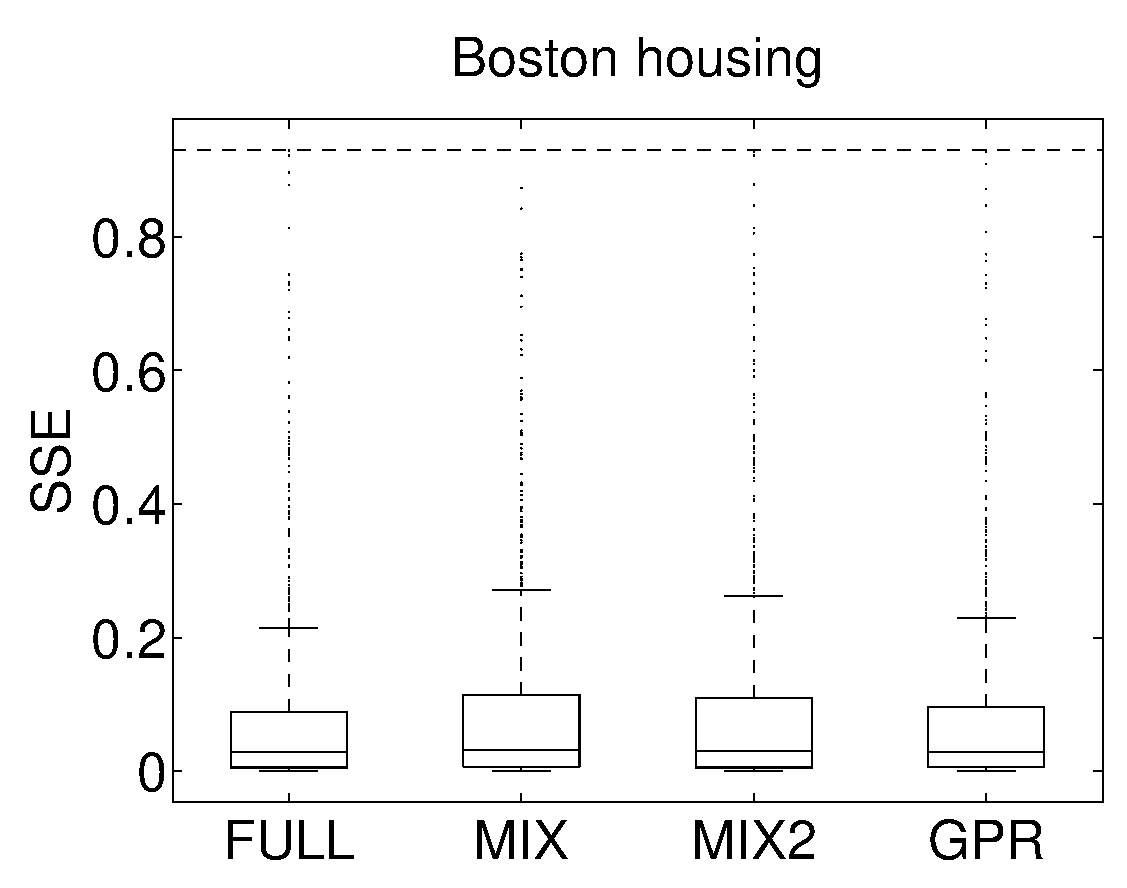
\includegraphics[scale=0.2]{figures/housing-smse.eps} &
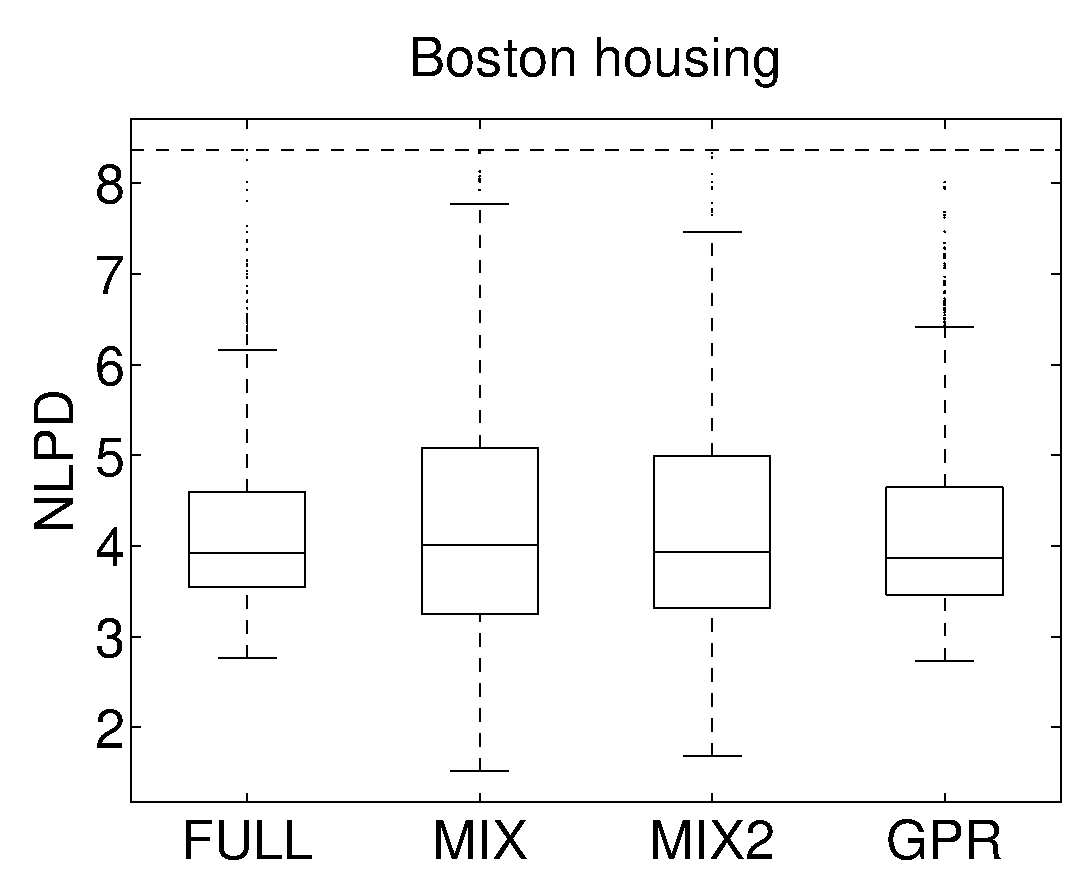
\includegraphics[scale=0.2]{figures/housing-nlpd.eps} \\
\end{tabular}
\caption{The distributions of SSE and NLPD of all methods on the regression task. Compared to the exact inference method GPR, the performance of AGP-FULL is identical while that of AGP-MIX and AGP-MIX2 are comparable.}
\label{fig:regression}
\end{figure*}

\subsection{Warped Gaussian processes (WGP)}
\begin{figure*}
\setlength{\tabcolsep}{0pt}
\begin{tabular}{cccc}
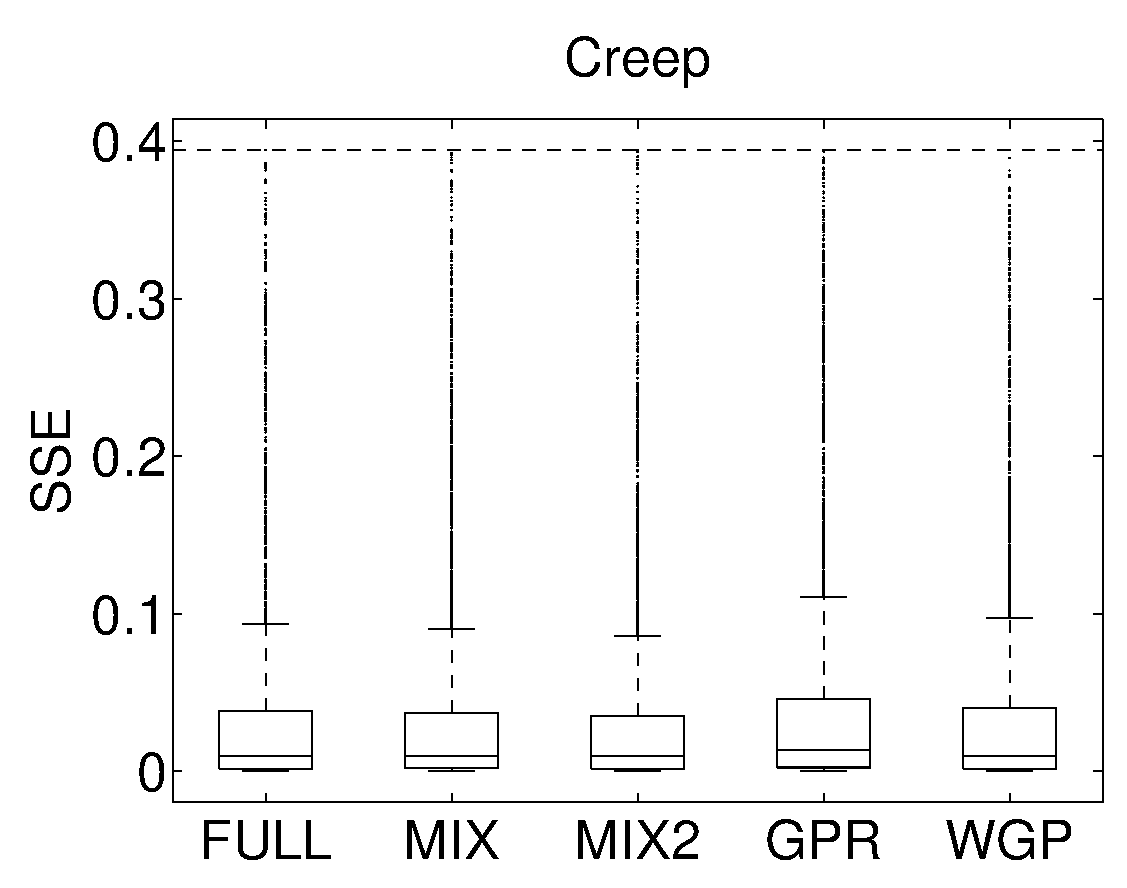
\includegraphics[width=0.25\linewidth]{figures/creep-smse.eps} &
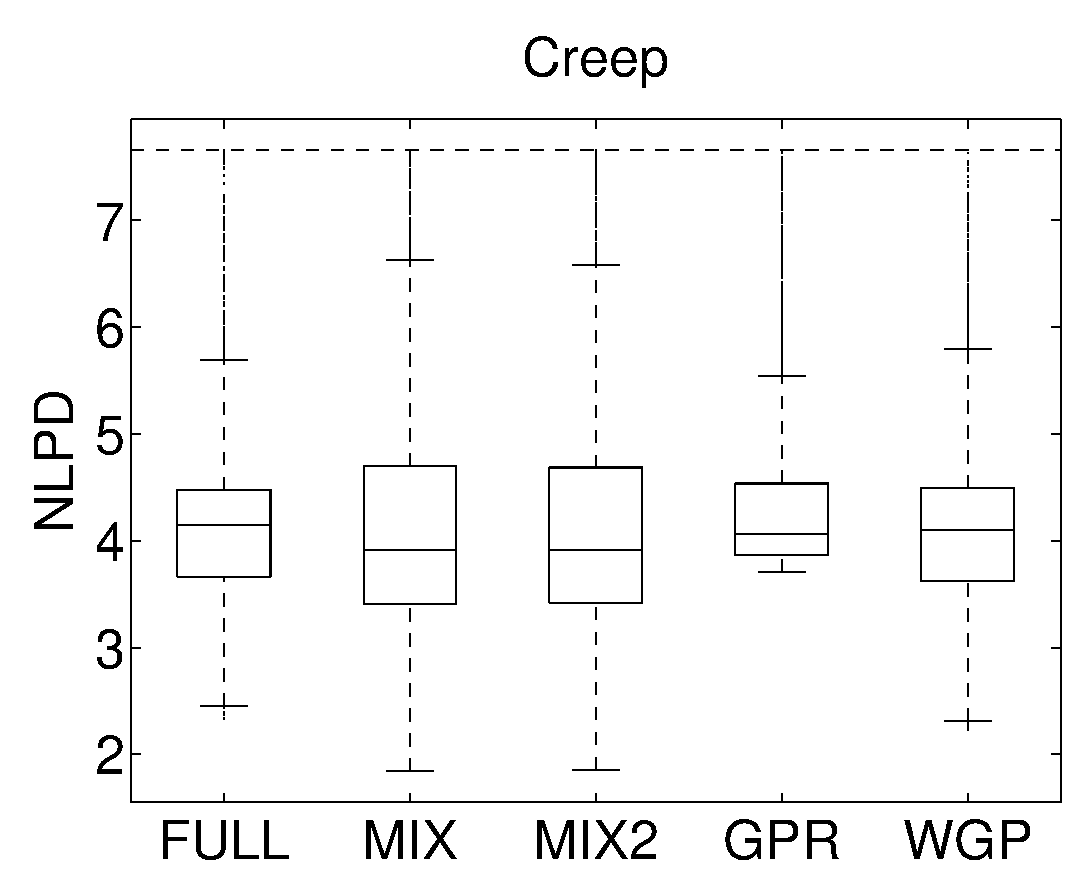
\includegraphics[width=0.24\linewidth]{figures/creep-nlpd.eps} &
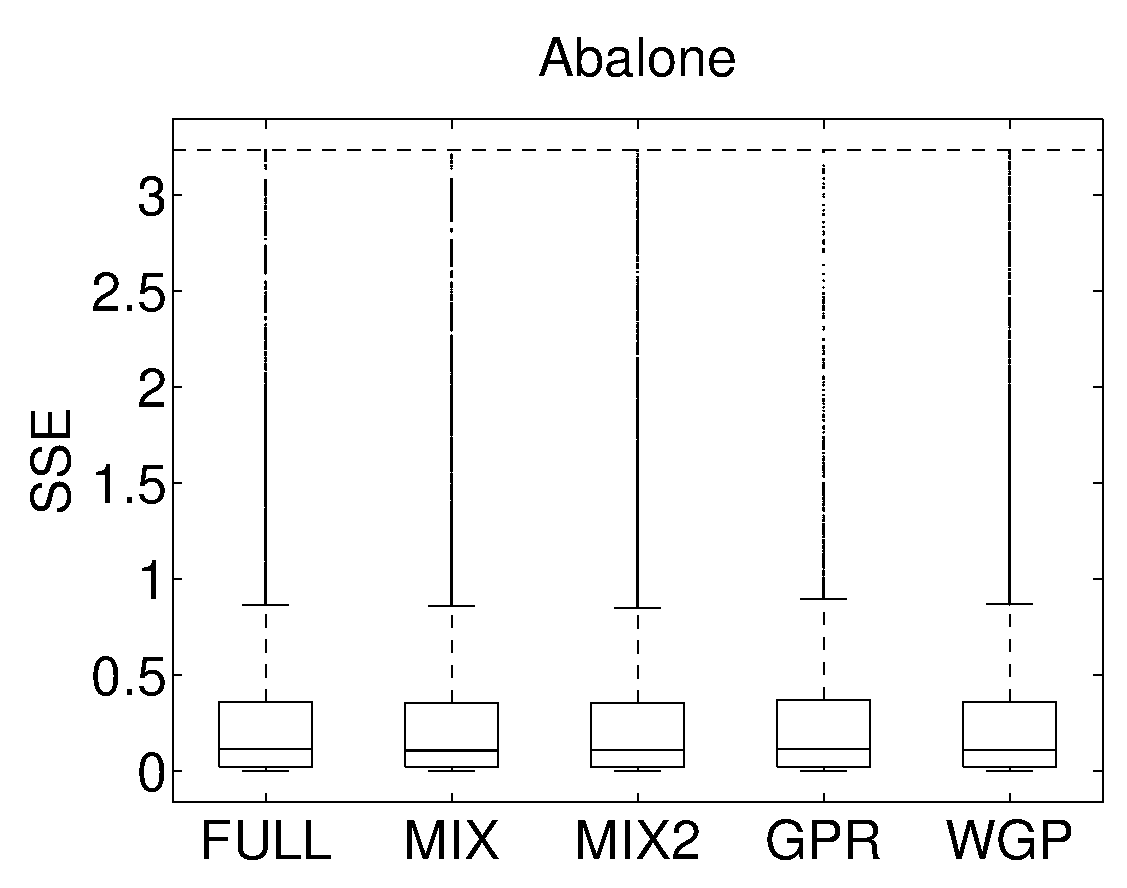
\includegraphics[width=0.25\linewidth]{figures/abalone-smse.eps} &
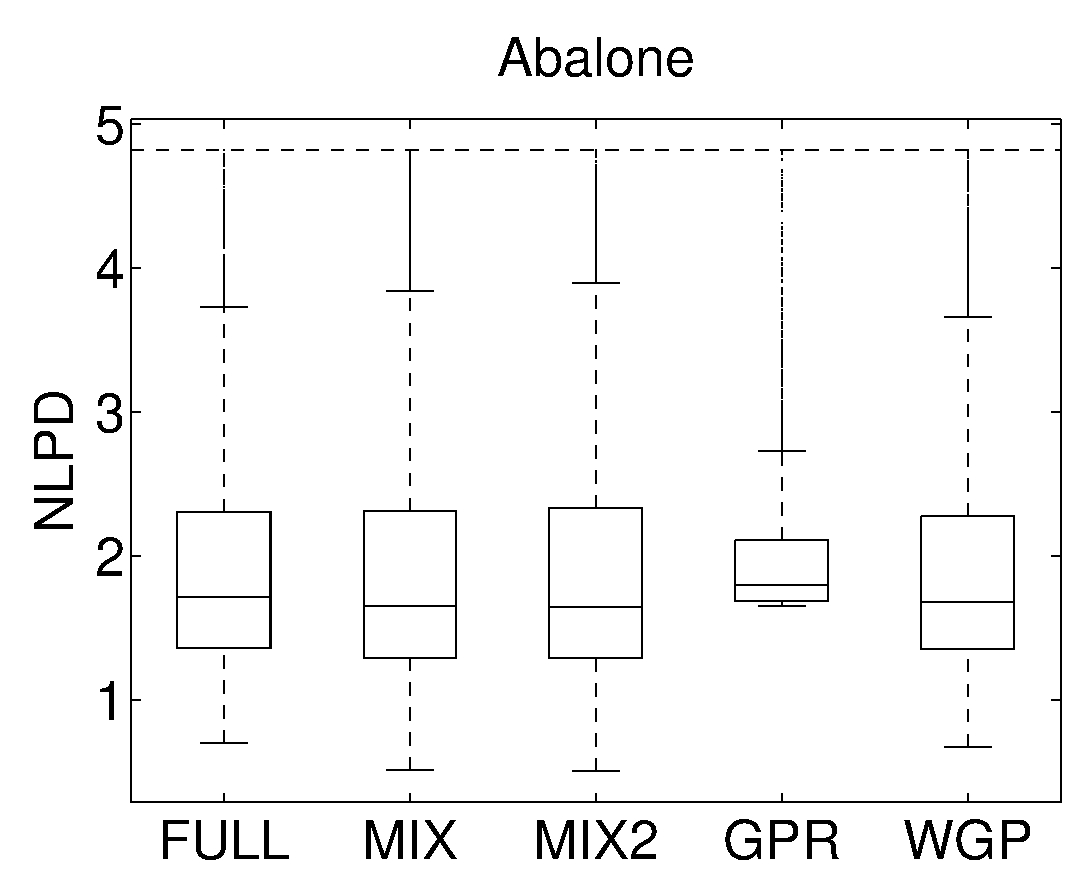
\includegraphics[width=0.24\linewidth]{figures/abalone-nlpd.eps} 
\end{tabular}
\caption{The distributions of SSE and NLPD of all methods on the regression task with warped GPs. 
The \agp \space methods ({\sc full}, {\sc mix} and {\sc mix2}) give comparable performance
to  exact inference with \wgp \space and slightly outperform \gpr \space which has  narrower ranges of predictive variances.}
\label{fig:warp}
\end{figure*}
%
The \wgp \space allows for non-Gaussian processes and non-Gaussian noises.
The likelihood for each target $y_n$ is attained by warping it through a nonlinear monotonic transformation $t(y)$ giving $p(y_n | f_n) = \nabla_{y_n} t(y_n) \Normal(t(y_n) | f_n, \sigma^2)$.
We used the same neural net style transformation %$t(y) = y + \sum_{i=1}^C a_i \tanh (b_i (y + c_i)), a_i, b_i \ge 0 \quad \forall i.$, where $a_i$, $b_i$, and $c_i$ parametrize $t(y)$
as in \cite{snelson2003warped}.
We fixed the warp parameters and used the same procedure for making analytical approximations to the predicted means and variances for all methods.

We compare with the exact implementation of \cite{snelson2003warped} %where the parameters are learned by optimizing the exact marginal likelihood.
and the standard GP regression (\gpr) on the Creep \cite{cole2000modelling} and Abalone \cite{uci2013} datasets.
%With Creep, the aim is to predict the creep rupture stress for steel given chemical composition and other inputs.
%With Abalone, the aim is to predict the age of abalone from various physical inputs.
The results in Figure \ref{fig:warp} show that the \agp \space methods give comparable performance to the exact  method \wgp \space and slightly outperform \gpr.  
The prediction by \gpr \space exhibits characteristically narrower ranges of predictive variances which can be attributed to its Gaussian noise assumption.

\subsection{Classification}
%For binary classification, the logistic likelihood $p(y_n = +1|f_n) = \frac{1}{1 + \exp(-f_n)}$ is chosen where $+1$ indicates the label of the positive class.
%The probability of the negative class with label $-1$ equals $1 - p(y_n = +1|f_n)$.
%For multiple classes, there are $C$ latent functions, $f_1$, $\hdots$, $f_C$, each associated with a different class.
%The latent function values at data point $n$ is collected into the vector $\f_{(n)} = [f_1(\x_n), \hdots, f_C(\x_n)]$ from which the softmax likelihood function can be constituted, 
%$p(\y_n | \f_{(n)}) = \frac{\sum_{i=1}^C \exp(y_{in} f_{in})}{\sum_{i=1}^C \exp(f_{in})}$.
%Here $f_{in} = f_i(\x_n)$ and $\y_n = \{y_{in}\}_{i=1}^C$ is a binary vector that has only an entry of 1 for the class label of the data point $n$.
%If we let that label be $c$, i.e., $y_{cn} = 1$ then the form given in Table \ref{tab:datasets} is recovered.
\begin{figure*}
\centering
\begin{tabular}{ccc}
\includegraphics[width=0.3\linewidth]{figures/classfication-errors.eps}  &
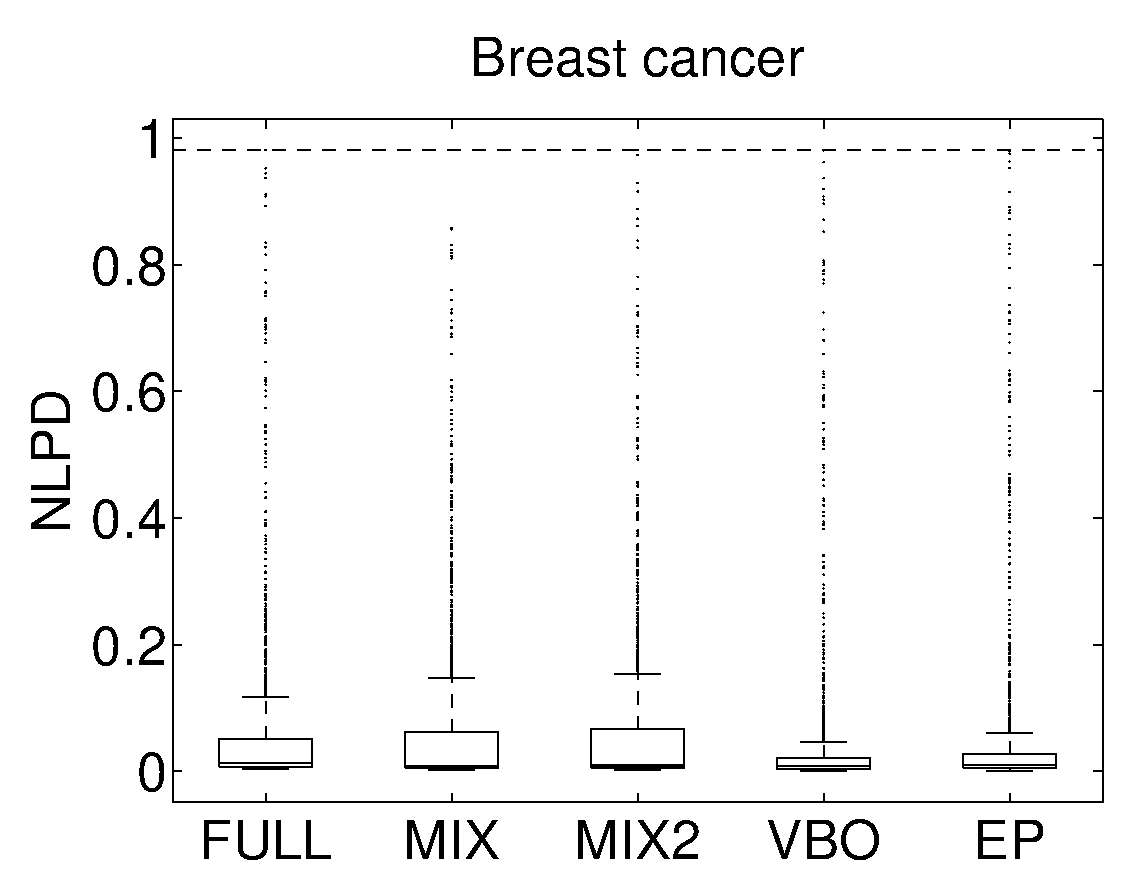
\includegraphics[width=0.3\linewidth]{figures/breast-nlpd.eps} &
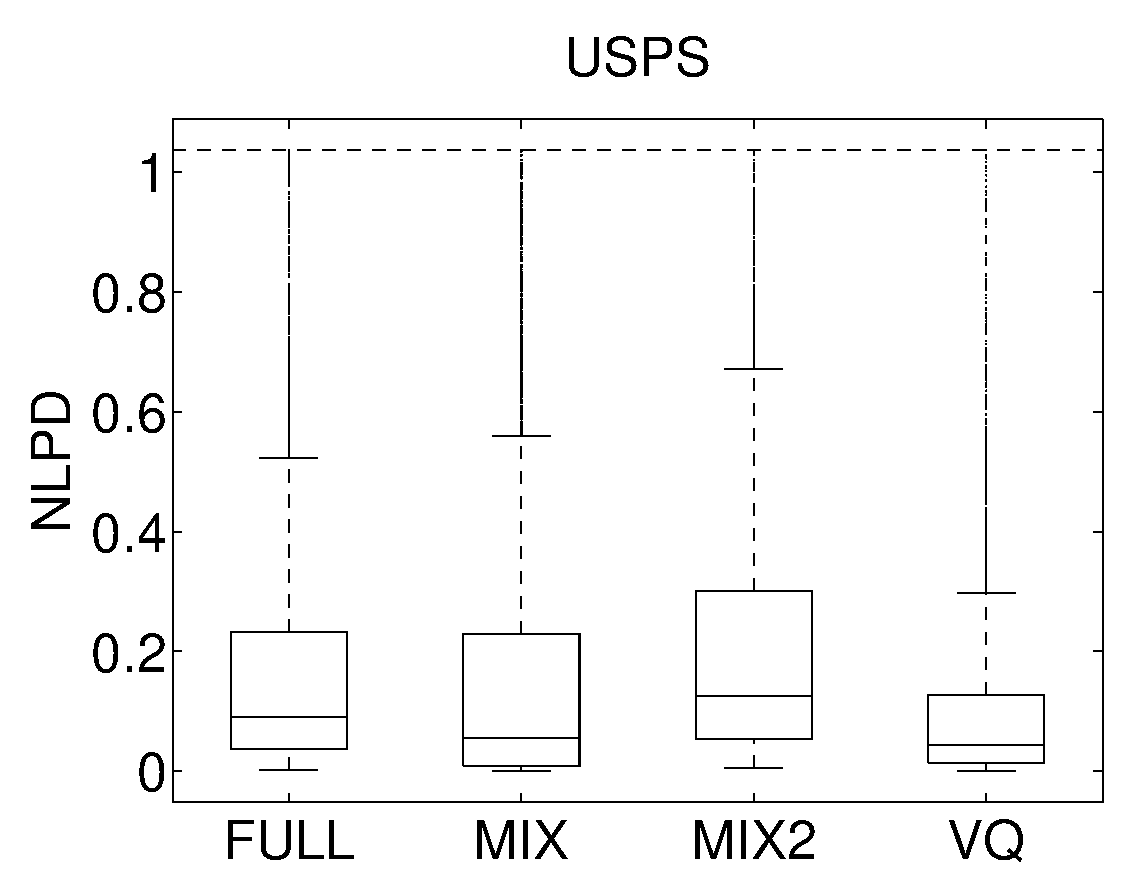
\includegraphics[width=0.3\linewidth]{figures/usps-nlpd.eps} 
\end{tabular}
\caption{\emph{Left plot}: classification error rates averaged over 5 runs (the error bars show two standard deviations). The \agp \space methods have classification errors comparable to the hard-coded implementations. \emph{Middle and right plots}: the distribution of NLPD of all methods on the binary and multi-class classification tasks, respectively. The hard-coded methods are slightly better than \agp.}
\label{fig:classification}
\end{figure*}

For binary classification, we use the logistic likelihood and experiment with the Wisconsin breast cancer 
 dataset \cite{uci2013}. %and the Ionosphere \cite{uci2013} datasets.
We compare with the variational bounds (\vbo) and the expectation propagation (\ep) methods.
%Note that \vbo \space is a local variational inference approach whose 
%ELBO is induced differently via a lower bound of the individual logistic likelihood. 
Details of \vbo \space and \ep \space can be found in  \cite{nickisch2008approximations}.
All  methods use the same analytical approximations when making prediction.

For multi-class classification, we use the softmax likelihood and experiment with a subset of the USPS dataset \cite{rasmussen-williams-book} containing the digits 4, 7, and 9.
We compare with a variational inference method  (\vq) which constructs the ELBO via a quadratic lower bound to the likelihood terms \cite{khan2012stick}.
Prediction is made by squashing the samples from the predictive distributions of the latent values at test points through the softmax likelihood for all methods.

The classification error rates and the NLPD are shown in Figure  \ref{fig:classification} for both tasks.
For binary classification, the \agp \space methods give comparable performance 
to the hard-coded implementations, \vbo \space and \ep. The latter is often considered the best approximation method for this task \cite{nickisch2008approximations}.
Similar results can be observed for the multi-class classification problem.
%The multi-modal posteriors \agpmixtwo \space do not seem to improve upon the uni-modal counterparts, suggesting that the true posterior may take the shape of a unimodal distribution.

We note that the running times of our methods are  comparable to that of the hard-coded methods.
For example, the average training times for \vbo, \ep, MIX, and FULL are 76s, 63s, 210s, and 480s respectively, on the Wisconsin dataset.

% previous figures with ionosphere
%\begin{figure*}
%\centering
%\begin{tabular}{c}
%\includegraphics[width=0.35\linewidth]{figures/classfication-errors.eps} 
%\end{tabular}
%\caption{Classification error rates on the binary and multi-class classification task. }
%\label{fig:classificationErrors}
%\end{figure*}

%\begin{figure*}
%\centering
%\begin{tabular}{ccc}
%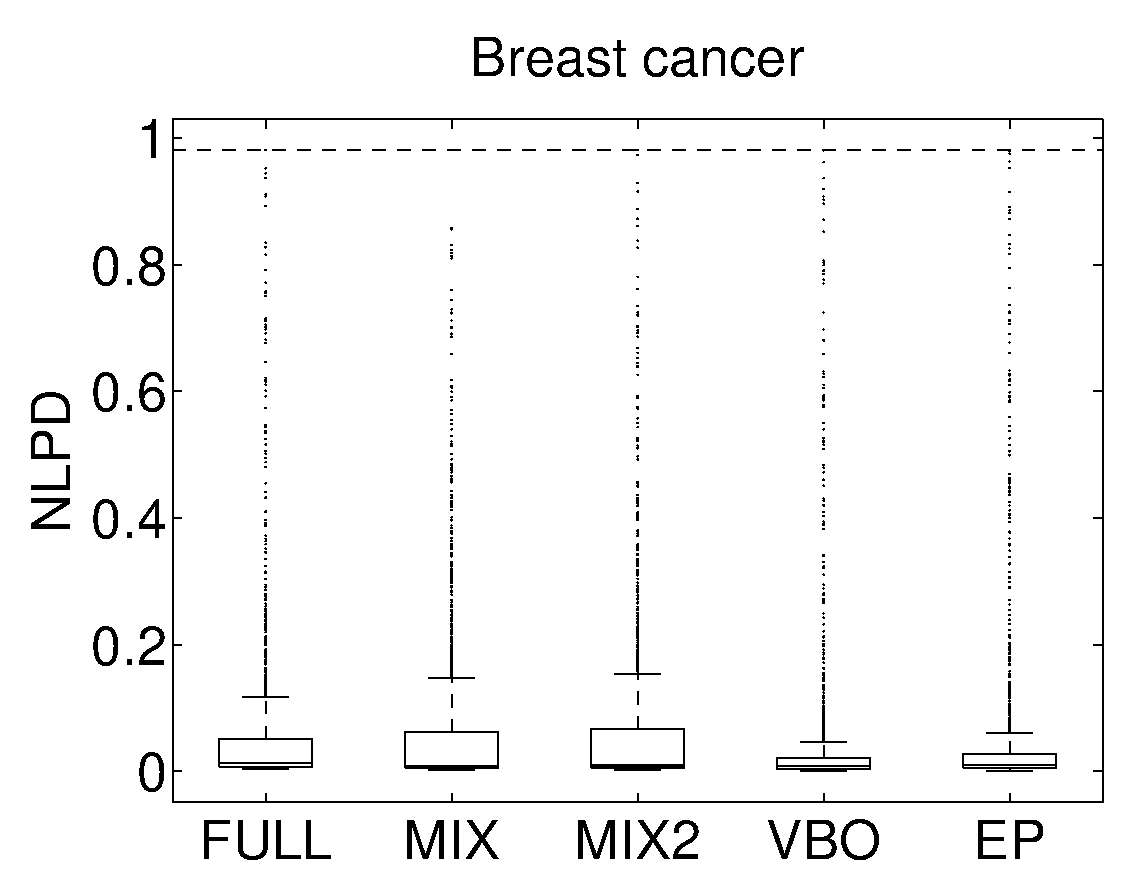
\includegraphics[width=0.25\linewidth]{figures/breast-nlpd.eps} &
%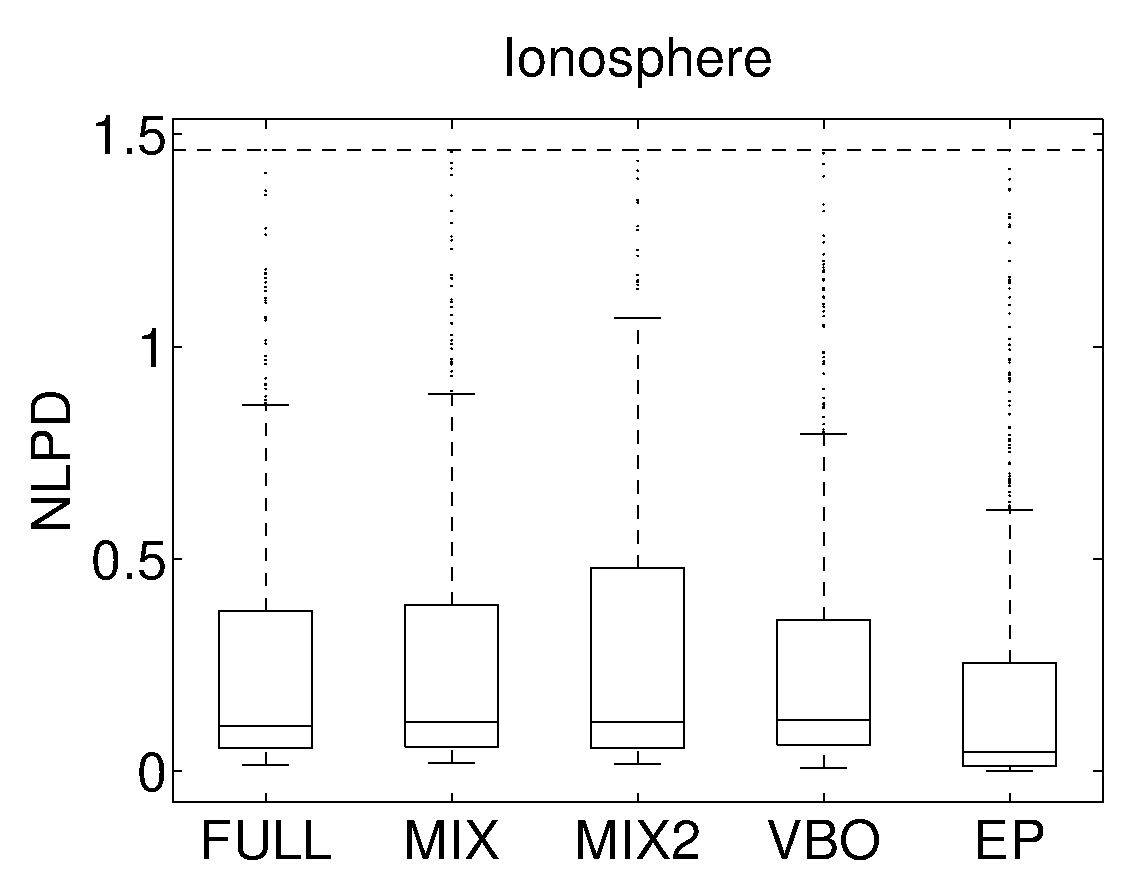
\includegraphics[width=0.25\linewidth]{figures/ionosphere-nlpd.eps} &
%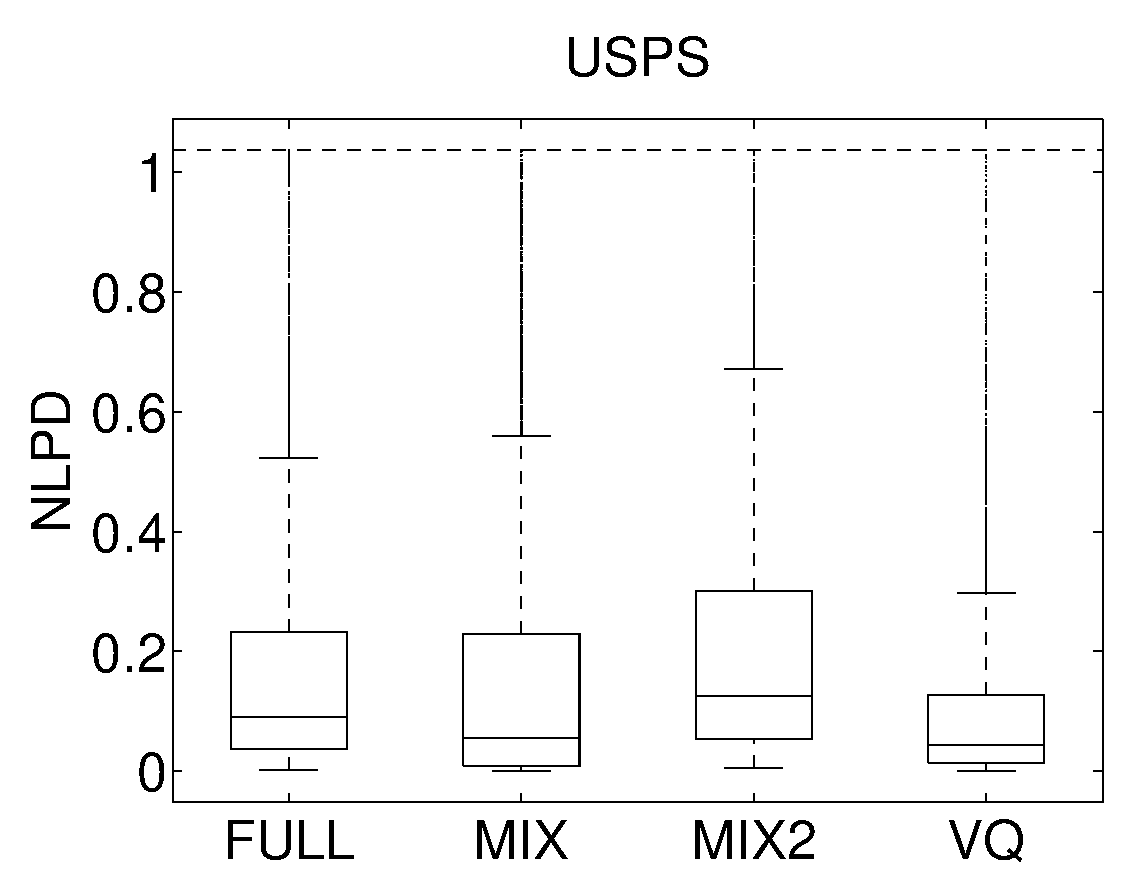
\includegraphics[width=0.25\linewidth]{figures/usps-nlpd.eps} 
%\end{tabular}
%\caption{Performance comparison on the binary and multi-class classification task. }
%\label{fig:classification}
%\end{figure*}

\subsection{Log Gaussian Cox process (LGCP) \label{sec:lgcp}}
The LGCP is an inhomogeneous Poisson process with the log-intensity function being a shifted draw from a Gaussian process.
Following \cite{murray2009elliptical}, we use the likelihood $p(y_n | f_n) = \frac{\lambda_n^{y_n} \exp(-\lambda_n)}{y_n!},$ where $\lambda_n = \exp(f_n + m)$ is the mean of a Poisson distribution and $m$ is the offset to the log mean. 
The data concerns  coal-mining disasters taken from a standard dataset for testing point processes \cite{jarrett1979note}.
The offset $m$ and the covariance hyperparameters are set to the same values as in \cite{murray2009elliptical}.
%The 191 events were placed into 811 bins of 50 days each. 
%The offset $m$ is set to $m = log(191/811)$ and the covariance hyperparameters fixed to $\sigma_f^2 = 1$ and $l = 13516$.
%The covariance hyperparameters are fixed to $\sigma_f^2 = 1$ and $l = 13516$.

We compare \agp \space with the  Hybrid Monte Carlo (\hmc, \cite{duane1987hybrid}) and 
elliptical slice sampling  (\ess, \cite{murray2009elliptical}) methods, where the latter is designed specifically for GP models.
We collected every $100$th sample for a total of $10$k samples after a burn-in period of $5$k samples; the  Gelman-Rubin potential scale reduction factors \citep{gelman1992inference} are used to check for convergence. 
%In Figure \ref{fig:loggcp}, the left plot shows the true event counts per 50 days during the given time period.
%The middle plot shows the posteriors by all methods.
The middle plot of Figure \ref{fig:loggcp} shows the posteriors learned by all methods.
 We see that the posterior by \agpfull \space is 
 similar to that 
by \hmc \ and \ess.
\agpmix \space obtains the same posterior mean but it underestimates the variance. 
%Note that the predictive mean of all methods will be the same as it does not depend on the variance of the posterior.
The right plot shows the speed-up factors of all methods against the slowest method \hmc. % -- the slowest method. which took $196$ minutes, in $\log_{10}$ scale.
The \agp \space methods run more than two orders of magnitude faster than \hmc, thus confirming the computational advantages of our method to the sampling approaches.
Training time was measured on a desktop with Intel(R) i7-2600 3.40GHz CPU with 8GB of RAM using Matlab R2012a.
\begin{figure*}
\centering
\begin{tabular}{ccc}
\includegraphics[width=0.3\linewidth]{figures/loggcp-intensity.eps} &
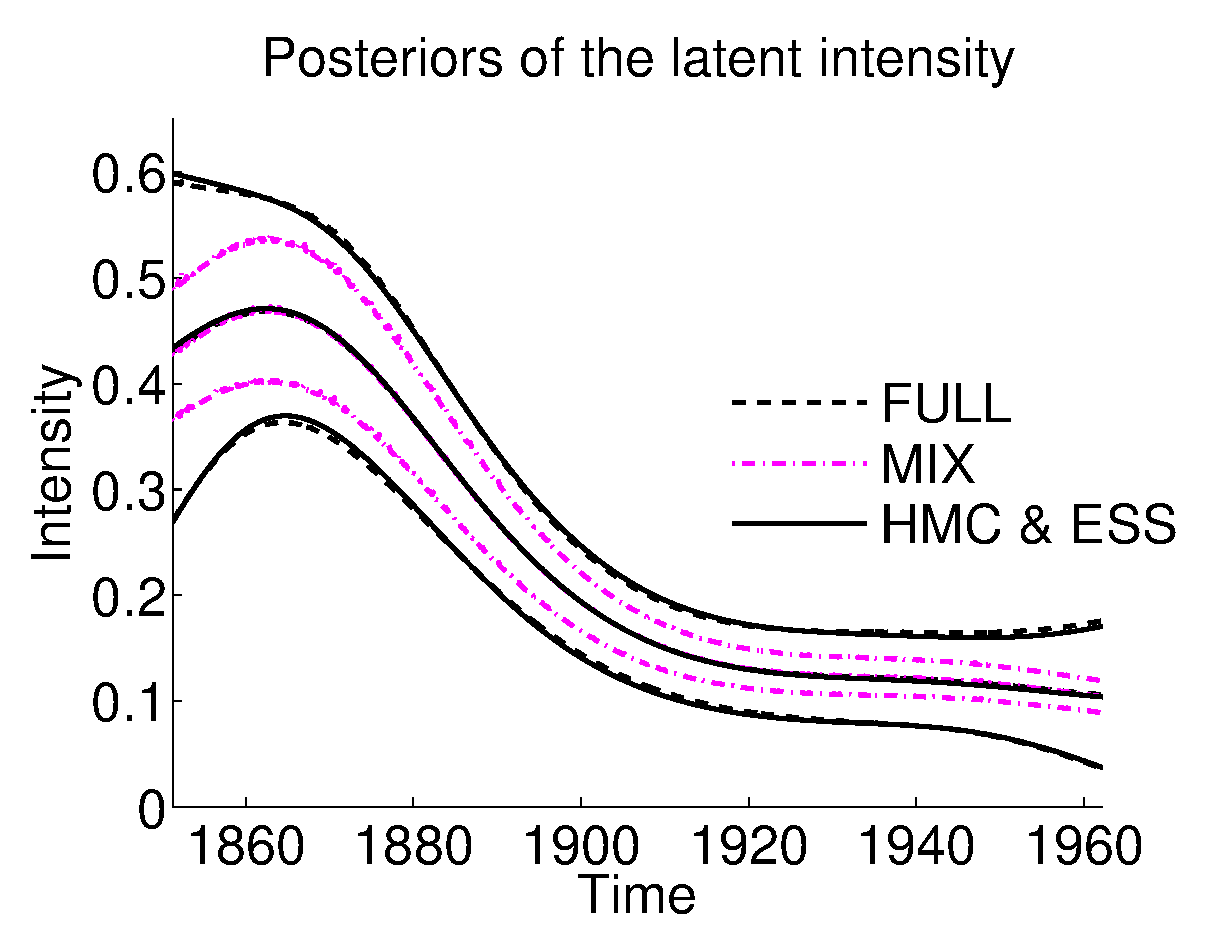
\includegraphics[width=0.3\linewidth]{figures/loggcp.eps} &
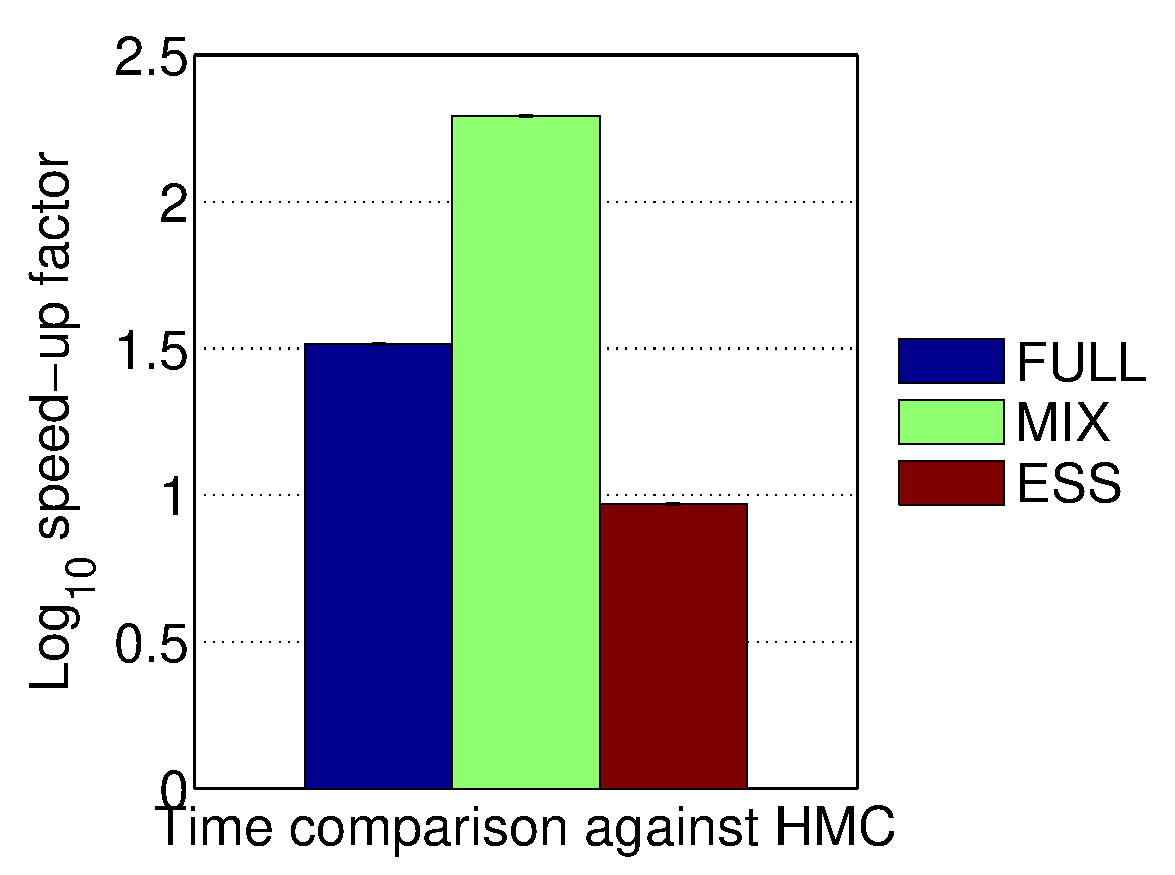
\includegraphics[width=0.3\linewidth]{figures/loggcp-time.eps}
\end{tabular}
\caption{\emph{Left plot}: the true event counts during the given time period. \emph{Middle plot}: the posteriors (estimated intensities) inferred by all methods. For each method, the middle line is the posterior mean and the two remaining lines enclose 90\% interval. \agpfull \space infers the same posterior as \hmc \space and \ess \space while \agpmix \space obtains the same mean but underestimates the variance. \emph{Right plot}: speed-up factors against the HMC method. The \agp \space methods run more than 2 orders of magnitude faster than the sampling methods. %The posterior distributions are virtually identical for the two sampling methods and the variational inference with full posterior. The diagonal posterior underestimates the variance, but the mean is the same as all other methods.
}
\label{fig:loggcp}
\end{figure*}

%\subsection{Toy Classification}
%Here I used a toy classifcation dataset (generated by the \textit{demoClassification} script in the GPML package). 
%The samples are generated from two Gaussian with different means and covariance.
%\paragraph{Prediction}
%The data and predictive probabilities of the test data points being in the positive class by the exact variational inference (\textbf{exactVB}), black box inference (\textbf{blackbox}), inference with a full Gaussian posterior (\textbf{fullGaussian}) and mixture of Gaussians posterior (\textbf{mixture}) are shown in Figure \ref{fig:toy}.
%It can be seen that black box inference fails to work (in fact the variance increases as the algorithm progresses).
%
%\begin{figure*}
%\centering
%\begin{tabular}{cc}
%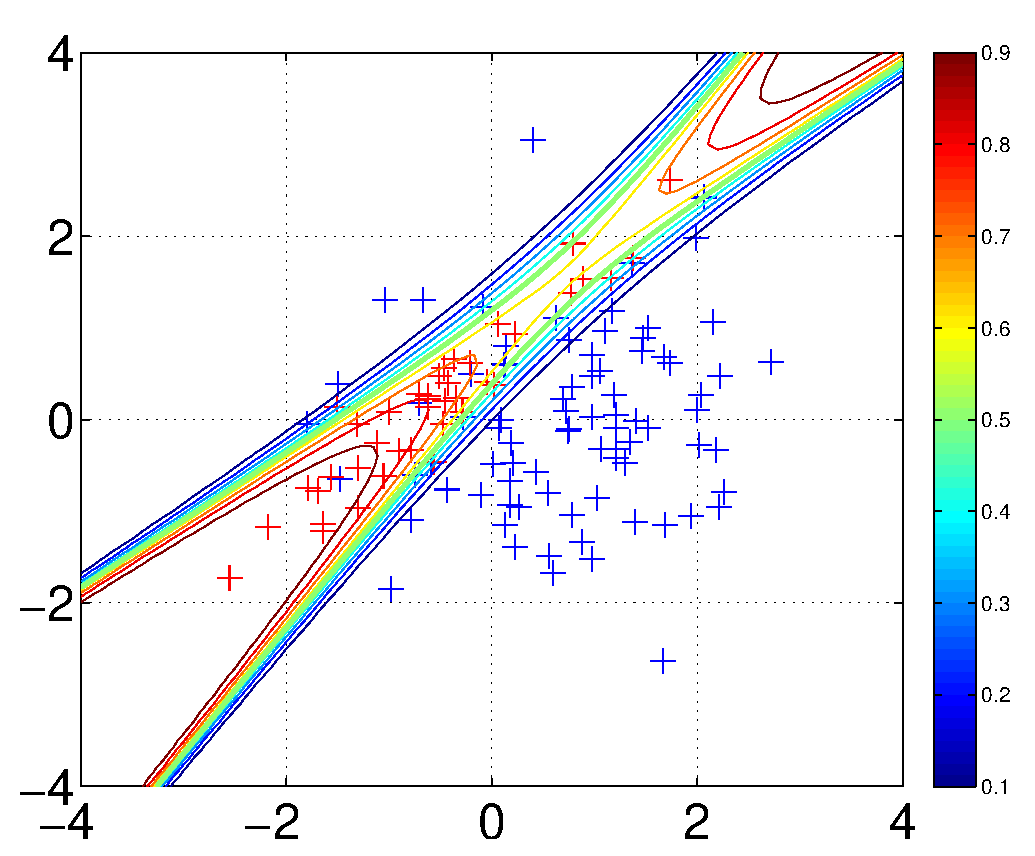
\includegraphics[scale=0.4]{figures/f6.eps} &
%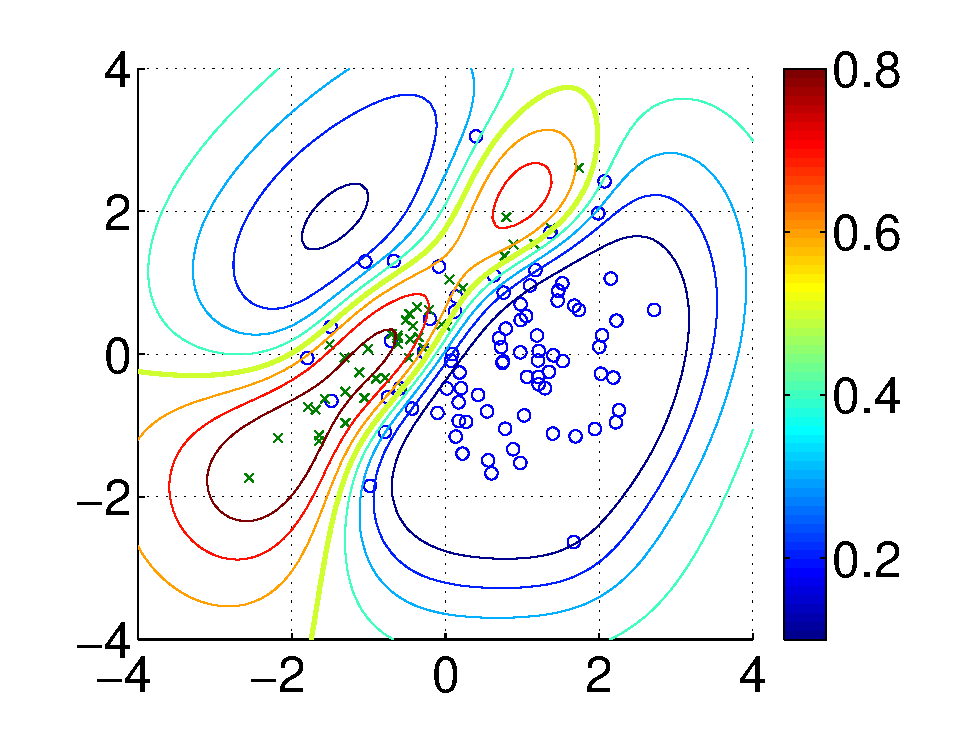
\includegraphics[scale=0.5]{figures/exactVB.eps} \\
%data & exactVB  \\
%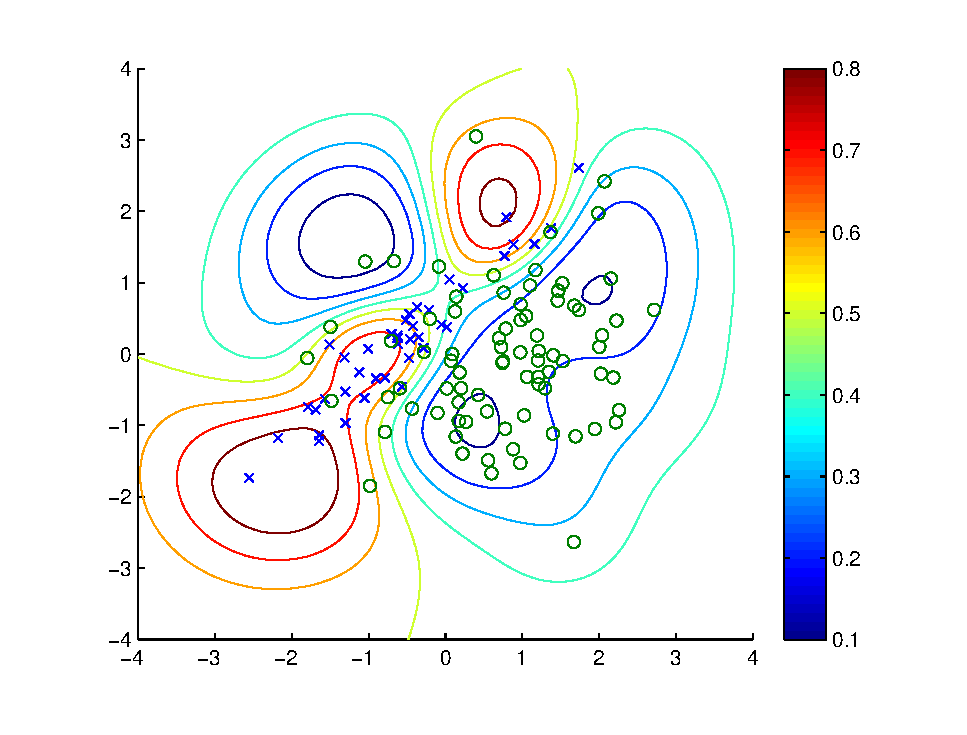
\includegraphics[scale=0.5]{figures/fullgaus-iter100-largelrate.eps} &
%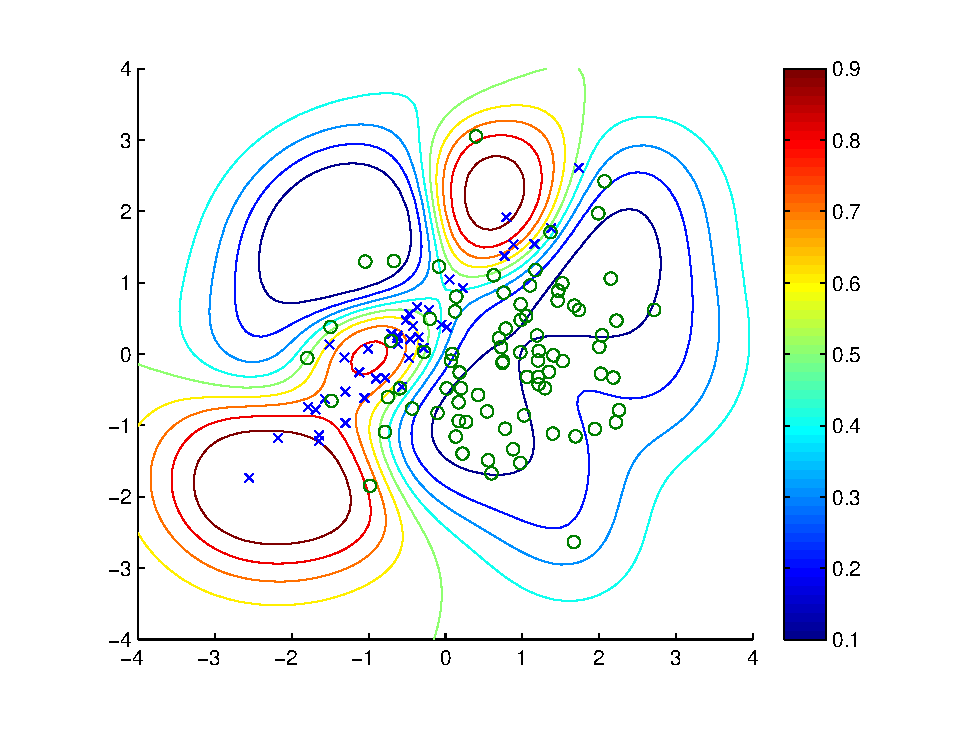
\includegraphics[scale=0.5]{figures/mixture-iter100-largelrate.eps} \\
%fullGaussian & mixture \\
%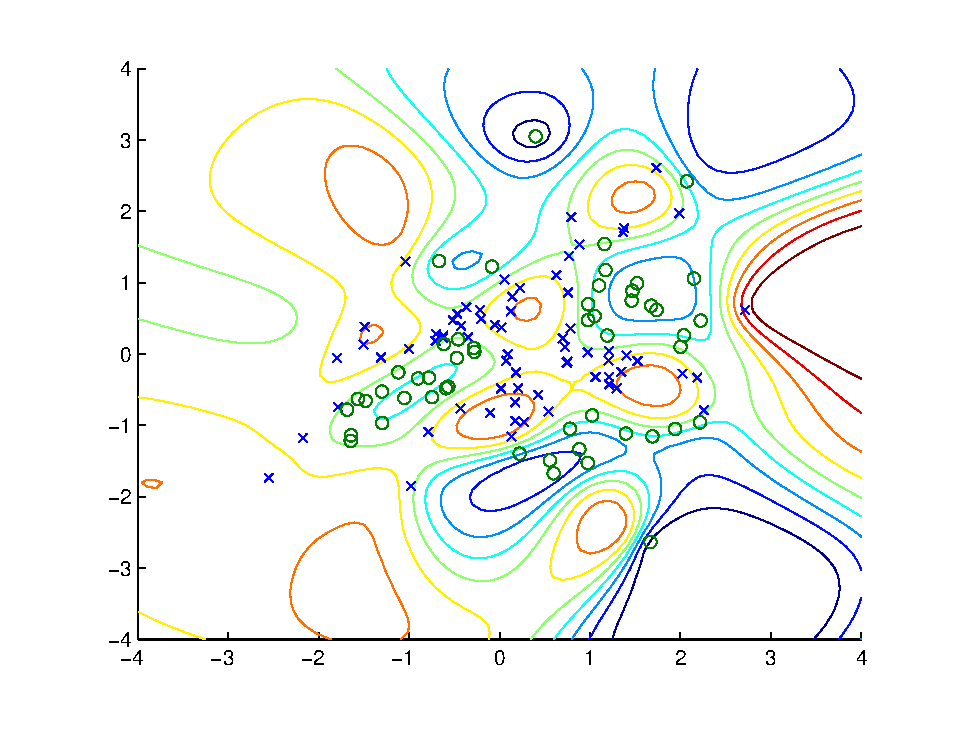
\includegraphics[scale=0.5]{figures/blackbox.eps} & \\
%blackbox
%\end{tabular}
%\caption{Data and the contour of predictive probability of data points being classified as positive. The dots are training data points. (The marker for the 2 classes of exactVB should be switched, but the contour means the same thing!)}
%\label{fig:toy}
%\end{figure*}
%
%\paragraph{Variances of the estimators}
%The average variances of the gradient estimators are $3$ and $1e4$ for the mixture (with one component) and  full Gaussian, respectively. The variance for black box inference is $1e8$ with 10,000 samples and $1e10$ with 2000 samples.
%It is clear that merely increasing the number of samples is not effective in reducing the variance.
%
%\paragraph{Training time}
%Training time for the mixture with one component (100 iterations) takes around 1 minute.
%Training time for full Gaussian (also with 100 iterations) is around 10 minutes.
%Training time for black box inference (also with 100 iterations) is around 20 minutes. The additional cost is due to sampling to estimate the gradient of the hyperparameters and also due to computing the entropy and cross-entropy which are analytic in our proposal.



\section{Discussion}
We have developed automated variational inference for Gaussian process models (AGP). 
AGP performs as well as the  exact or hard-coded implementations when testing on five models using six real world datasets.
%
AGP has the potential to be a powerful tool for  GP practitioners and researchers 
when devising models for new or existing problems for which variational inference 
is not yet available.
%The process of investigating a new GP model typically involves tasks 
%such as proposing a new functional form for the likelihood; 
%restraining the domain of the latent function via a transformation; 
%or combining the latent functions to create novel correlations.
%With AGP, these tasks can all be carried out with little effort -- simply by implementing a new likelihood function.
In the future we will address the scalability of 
AGP to deal  with very large datasets.


\subsubsection*{Acknowledgements}
NICTA is funded by the Australian Government through the Department of Communications and the Australian Research Council through the ICT Centre of Excellence Program. 

\small
\bibliography{references}
\bibliographystyle{unsrt}

\end{document}
